\documentclass{beamer}
%\usepackage{xcolor}
%\usepackage{graphicx}

%\usepackage{amsmath}
%\usepackage{amsfonts}
\usepackage{bm}
%\usepackage{natbib}
%\usepackage{amssymb,amsthm}
%\usetheme{Gerrish}
%\usepackage[mathcal]{euscript}   % for script letters
%\usepackage{array}
%\usepackage{wrapfig}
%\usepackage{multirow}

\setbeamertemplate{navigation symbols}{}
\setbeamertemplate{outlinem}{}

%\bibliographystyle{icml2012}
\bibliographystyle{apalike}

\newcommand{\z}{\textbf{z}} 
\newcommand{\W}{\textbf{W}}
\newcommand{\mv}{\tilde{m}} 
\newcommand{\vv}[0]{\tilde{V}}
\newcommand{\w}{\textbf{w}}
\newcommand{\vphi}{\phi}
\newcommand{\bv}{\tilde{\beta}}
\newcommand{\bb}{\beta}
\newcommand{\lv}{\tilde{l}}
\newcommand{\vlv}{\sigma^2_{l}}
\newcommand{\vd}{\sigma^2_{d}}
\newcommand{\vbv}{\sigma^2}
\newcommand{\stdnorm}[1]{\mathcal{N}\left(#1\right)}


\newcommand{\tr}[0]{\mbox{Tr}}
\newcommand{\expectq}[1]{\mathbb{E}_q\left[#1\right]}
\newcommand{\expectqnoarg}[0]{\mathbb{E}_q}
\newcommand{\defn}[0]{:=}
\newcommand{\partl}[2]{\frac{\partial #1}{\partial #2}}


\title{Latent-variable models of influence and decision-making}
 \subtitle{}
 \date{8 January 2013}
 \author{ Sean Gerrish \\
   Princeton University \\
   Computer Science Department }

\setbeamersize{text margin left=0cm}

\begin{document}
\frame{\titlepage}

% \frame {

%   \large ``So far there have been only scattered examples of the
%   potential of mining social media.''
  
% \vspace{10pt}
% \tiny
% \hspace{80pt} \textcolor{gray}{”Government Aims to Build a ‘Data Eye in the Sky’”. The New York Times. Feb 11, 2011}

% }

\frame {
  \vspace{10pt}
  \small
  \emph{Most of the Big Data surge is data in the wild -- unruly stuff like words, images and video on the Web... It is called unstructured data and is not typically grist for traditional databases.}

% \vspace{30pt}
% ... At the forefront are the rapidly advancing techniques of artificial intelligence like natural-language processing, pattern recognition and machine learning.''
\vspace{5pt}
\tiny \hspace{100pt} \textcolor{gray}{“The Age of Big Data.” The New York Times. Feb 11, 2012}
\begin{center}
  
\includegraphics[width=0.84\textwidth,height=0.3\textheight]{figs/news.jpg} \\
\end{center}

\small
\emph{The most optimistic researchers believe that these
  storehouses of “big data” will for the first time reveal
  sociological laws of human behavior -- enabling them to predict
  political crises, revolutions and other forms of social and economic
  instability, just as physicists and chemists can predict natural
  phenomena.}

\vspace{5pt}
  \tiny \hspace{100pt} \textcolor{gray}{”Government Aims to Build a ‘Data Eye in the Sky’”. The New York Times. Feb 11, 2011}

}

\frame {
  \frametitle{Overview}
\large  Machine learning is making it possible to understand what is going on in large collections of text documents.
\large
\vspace{20pt}
  \begin{itemize}
  \item Understanding patterns of events in collections of text
    \begin{itemize}
    \item How to discover international relations using news articles
    \item How to find influential text documents
    \end{itemize}
  \vspace{20pt}
  \item Understanding government with latent variable models of text
    \begin{itemize}
    \item Understanding lawmakers' issue preferences
    \item How to predict votes on new bills
    \end{itemize}
  \end{itemize}
}

\frame {
  \frametitle{Overview}
\large  Machine learning is making it possible to understand what is going on in large collections of text documents.
\large
\vspace{20pt}
  \begin{itemize}
  \item Understanding patterns of events in collections of text
    \begin{itemize}
    \item How to discover international relations using news articles
    \item \textcolor{gray}{How to find influential text documents}
    \end{itemize}
  \vspace{20pt}
  \item Understanding government with latent variable models of text
    \begin{itemize}
    \item Understanding lawmakers' issue preferences
    \item \textcolor{gray}{How to predict votes on new bills}
    \end{itemize}
  \end{itemize}
}

\frame {
 \frametitle{}
 \center
 
\includegraphics[width=1.1\textwidth]{figs/bad_headlines.jpg}
}

\frame {
 \frametitle{}
 \center
 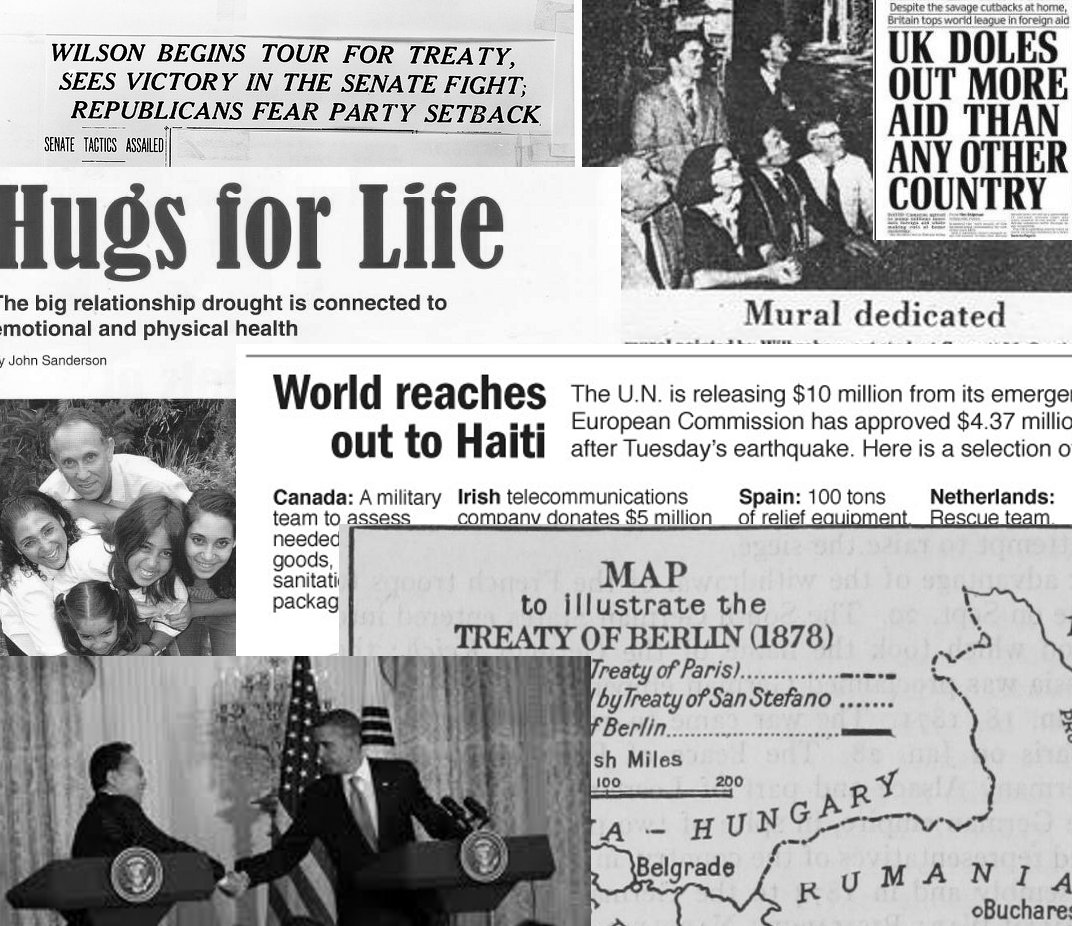
\includegraphics[width=1.1\textwidth]{figs/good_headlines.jpg}
}

\frame {
 \frametitle{A model of foreign relations sentiment}
 \Large Our goal is to automatically create a history of the relationship between countries from newspaper articles.
 \begin{itemize}
   \item Collect a bunch of newspaper articles on world news.
   \item Find snippets of text that mention pairs of countries.
   \item Label interactions between pairs of countries:
   \begin{itemize}
     \normalsize
     \item Labels from Amazon Mechanical Turk workers
     \item Correlates of War and Issue Correlates of War
   \end{itemize}
   \item Use these labels to fit a \emph{spatial} model of the
     sentiment between different countries. \\
     \vspace{20pt}
     \tiny \textcolor{gray}{MTurk:  \cite{chang:2009}} \\
     \vspace{10pt}
     \tiny \textcolor{gray}{CoW: \cite{sarkees:2010,hensel:2001}} \\
     \vspace{2pt}
     \tiny \textcolor{gray}{Spatial: \cite{chang:2009,hoff:2002,clinton:2004,martin:2002,gartzke:1998}}
     \normalsize
 \end{itemize}
}

\frame {
  \frametitle{Labeling sentiment: typical task}
  \center
  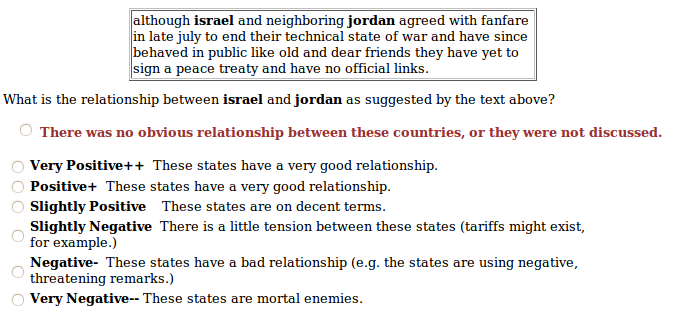
\includegraphics[width=1.1\textwidth]{figs/mturk_screenshot.png}
}

\frame {
  \frametitle{Correlates of War}
  \center
  \normalsize
  \begin{itemize}
  \item The \textbf{Correlates of War} \\
    \emph{seeks to facilitate the
    collection, dissemination, and use of accurate and reliable
    quantitative data in international relations}
    \cite{cow_webpage:2012}.  \\
    \vspace{1cm}
  \item The \textbf{Issue Correlates of War} \\
    \emph{is a research
    project that is collecting systematic data on contentious issues
    in world politics} \cite{icow_webpage:2012}
    \end{itemize}
}

\frame {
 \frametitle{Sentiment and news articles: text regression}
 \tiny
 \vspace{-20pt}
 \begin{center}
   \textcolor{gray}{\cite{kogan:2009}}
 \end{center}
 \vspace{10pt}
 \huge
 \begin{align*}
 s_d = \bm w_d^T \bm \beta + \varepsilon
 \end{align*}
 \Large
 \vspace{10pt}
 \begin{itemize}
   \item $\bm w_d \in \mathbb{R}^V$ is the text of a news paragraph \\
   \item $s_d \in \mathbb{R}$ is the ``sentiment'' between two
     countries \\
     \begin{itemize}
       \large
       \item Mechanical Turk labels $\{ -5, -3, -1,
         \textcolor{white}{-}1, \textcolor{white}{-}3,
         \textcolor{white}{-}5 \}$ \\
         \large
       \item Correlates of War labels $\{ -5, -1, 0.1\}$ \\
     \end{itemize}
         \Large
   \item $\bm \beta \in \mathbb{R}^V$ is the ``weight'' of each word
 \end{itemize}
}

\frame {
 \frametitle{Sentiment and news articles: text parameter \LARGE $\beta$ }
% \hspace{-36pt}
% \begin{tabular}{cc}
    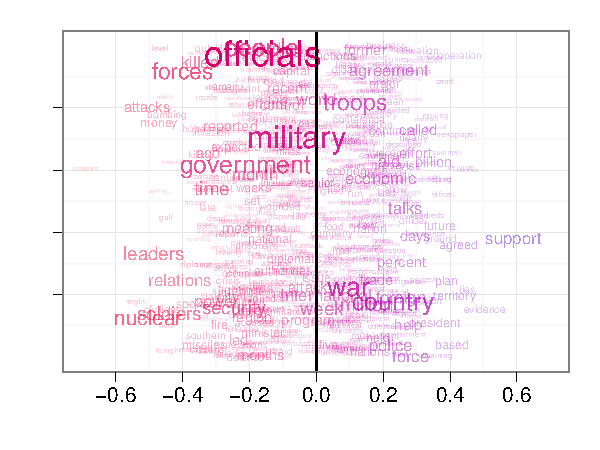
\includegraphics[width=1.0\textwidth]{figs/mturk_sample_words.pdf}
% &   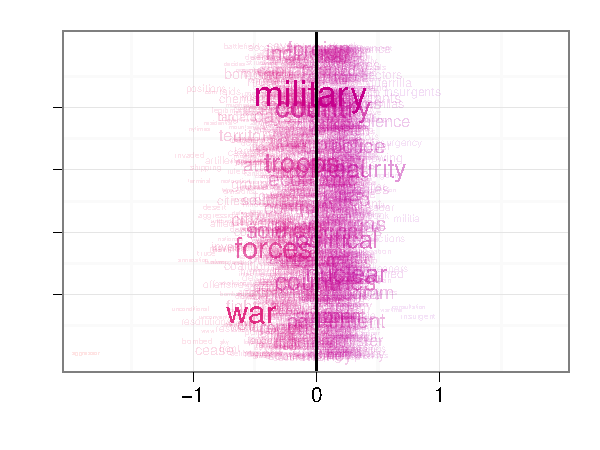
\includegraphics[width=0.4\textwidth]{figs/cow_sample_words.pdf} 
 %   \end{tabular}
}

% \frame {
%  \frametitle{A spatial model of foreign relations sentiment}
%  \Large This work develops a model of the sentiment between countries over time.
%  \begin{itemize}
%    \item It models dynamic relationships in an interpretable way
%    \item It infers sentiment from printed media
%    \item Sentiment is defined by Mechanical Turkers
%  \end{itemize}
% }

\frame {
 \frametitle{Countries take latent positions $\bar x_{ct}$ over time}
 \center
 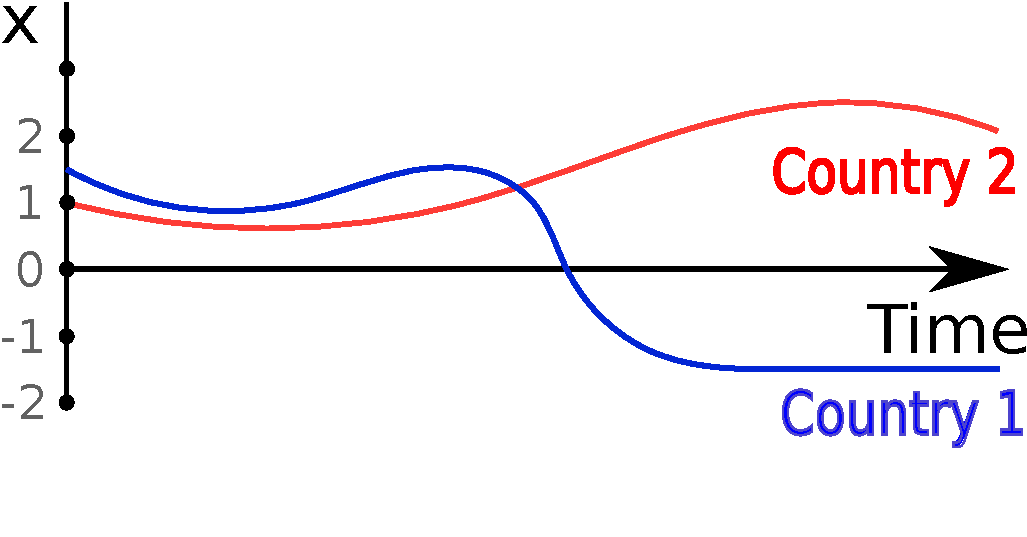
\includegraphics[width=0.7\textwidth]{figs/two_countries.pdf} \\
 \huge
 \begin{eqnarray*}
   \textcolor{blue}{\bar x_{c,t}} | \textcolor{blue}{\bar x_{c,t-1}} \sim N(\textcolor{blue}{\bar x_{c,t-1}}, \sigma_K^2) \nonumber \\
 \end{eqnarray*}
}

\frame {
 \frametitle{The relationship between countries is observed in the news.}
 \center
 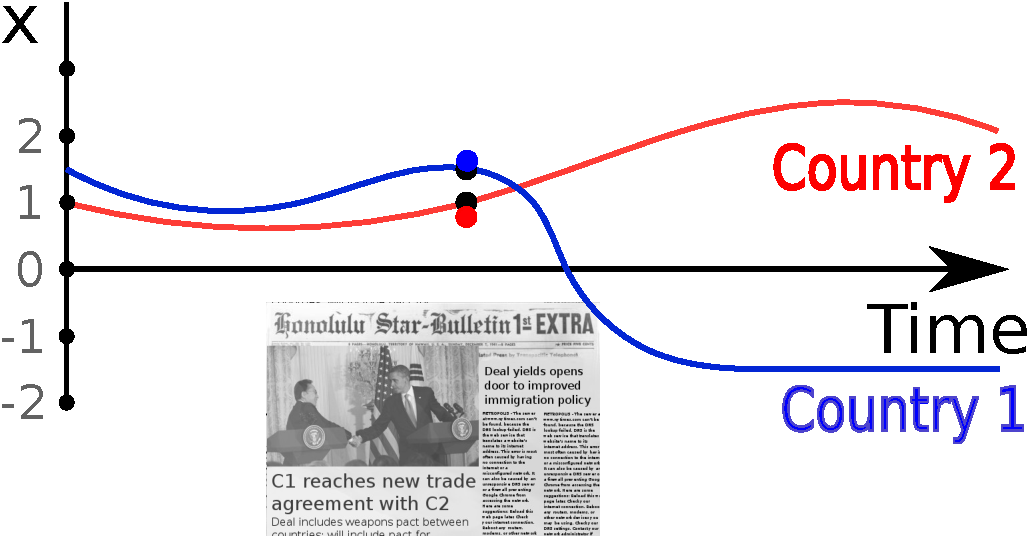
\includegraphics[width=0.7\textwidth]{figs/two_countries_time1.pdf}
 \center
 \Large
 \begin{eqnarray*}
  \textcolor{blue}{x_{c_1,d}} & \sim & N(\textcolor{blue}{\bar x_{c_1, t}}, \sigma_D^2) \nonumber \\
  \textcolor{red}{x_{c_2,d}} & \sim & N(\textcolor{red}{\bar x_{c_2, t}}, \sigma_D^2) \nonumber \\
  \mbox{Sentiment } s_d & := & \mathcal{F}( \textcolor{blue}{x_{c_1,d}},
  \textcolor{red}{x_{c_2,d}}) \nonumber \\
%  \mbox{For example: } \mathcal{F}( \textcolor{blue}{x_{c_1,d}},
 % \textcolor{red}{x_{c_2,d}} ) & = & \textcolor{blue}{x_{c_1,d}}^T
 % \textcolor{red}{x_{c_2,d}} \nonumber \\
 \end{eqnarray*}
}

\frame {
\frametitle{Example link functions $\mathcal{F}$}
\center
%\begin{tabular}{ll}
\vspace{-15pt}
\begin{itemize}
  \item \textbf{intercept / inner product:} \hspace{10pt} $y_1 + y_2 + \bm z_{1}^T \bm
  z_{2}$ \\
  \vspace{15pt}
  \item \textbf{intercept / distance:} \hspace{36pt} $y_1 + y_2 - \log(|| $\textbf{$\bm z_{1}$}$ - $\textbf{$\bm
 z_{2}$}$ ||_2^2 + 1)$ \\
%\end{tabular} \\
\end{itemize}
\vspace{20pt}
Where $\bm z_1, \bm z_2$ are vectors and $y_1, y_2$ are scalars
contained in $\bm x_1$ and $\bm x_2$.
}

\frame {
 \frametitle{The relationship between countries is observed in the news}
 \center
 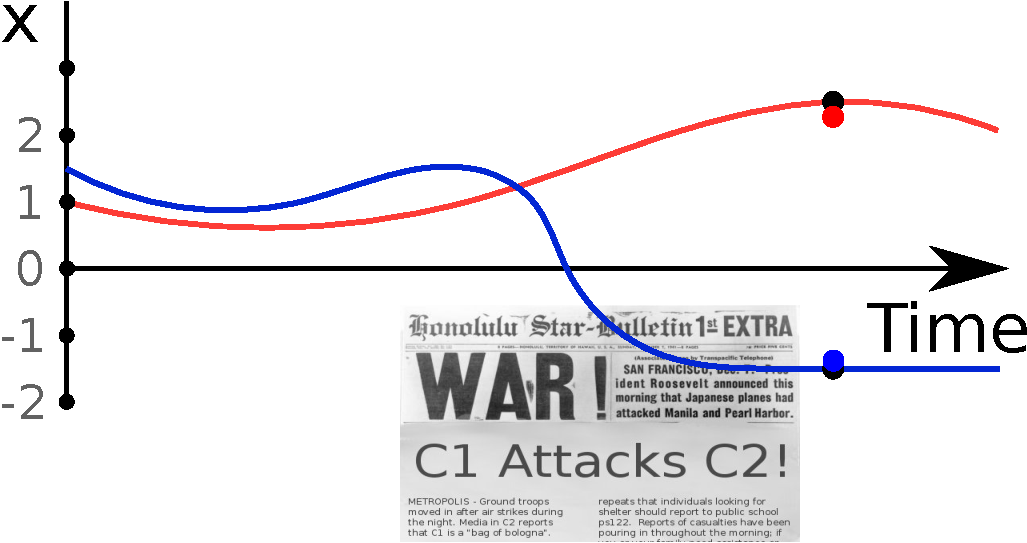
\includegraphics[width=0.7\textwidth]{figs/two_countries_time2.pdf}
 \LARGE
 \center
 \begin{eqnarray*}
  \textcolor{blue}{x_{c_1,d}} & \sim N(\textcolor{blue}{\bar x_{c_1, t}}, \sigma_D^2) \nonumber \\
  \textcolor{red}{x_{c_2,d}} & \sim N(\textcolor{red}{\bar x_{c_2, t}}, \sigma_D^2) \nonumber \\
  \mbox{Sentiment } s_d & := y_1 + y_2 -\log(1 + || \textcolor{blue}{z_{c_1,d}} - \textcolor{red}{z_{c_2,d}}||_2^2) \nonumber \\
 \end{eqnarray*}
}

\frame {
  \frametitle{The relationship between countries over time}
  \begin{center}
    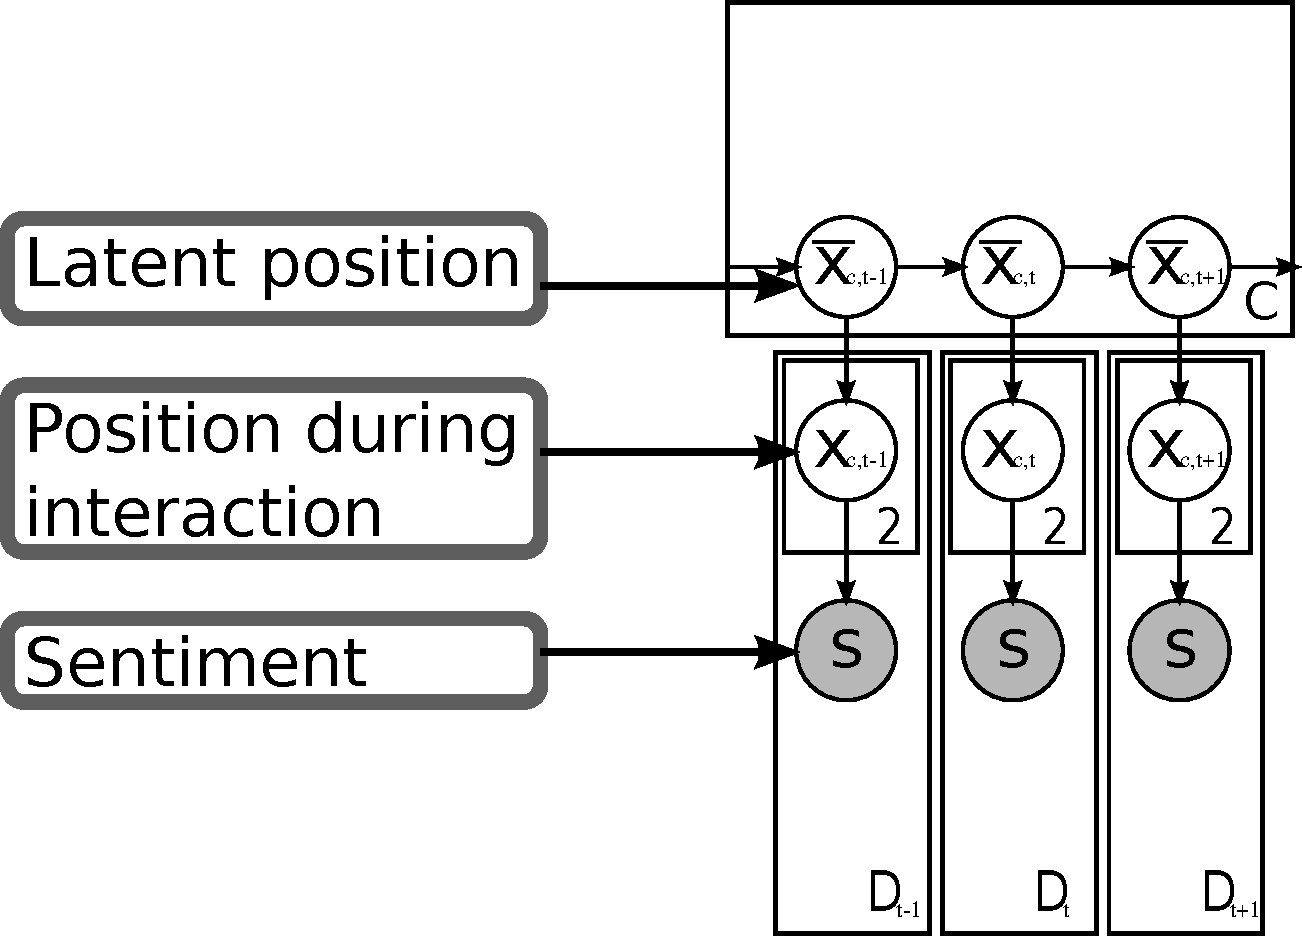
\includegraphics[width=0.8\textwidth]{figs/countries_gm_bare.pdf}
  \end{center}
}

\frame {
  \frametitle{The relationship between countries over time}
  \begin{center}
    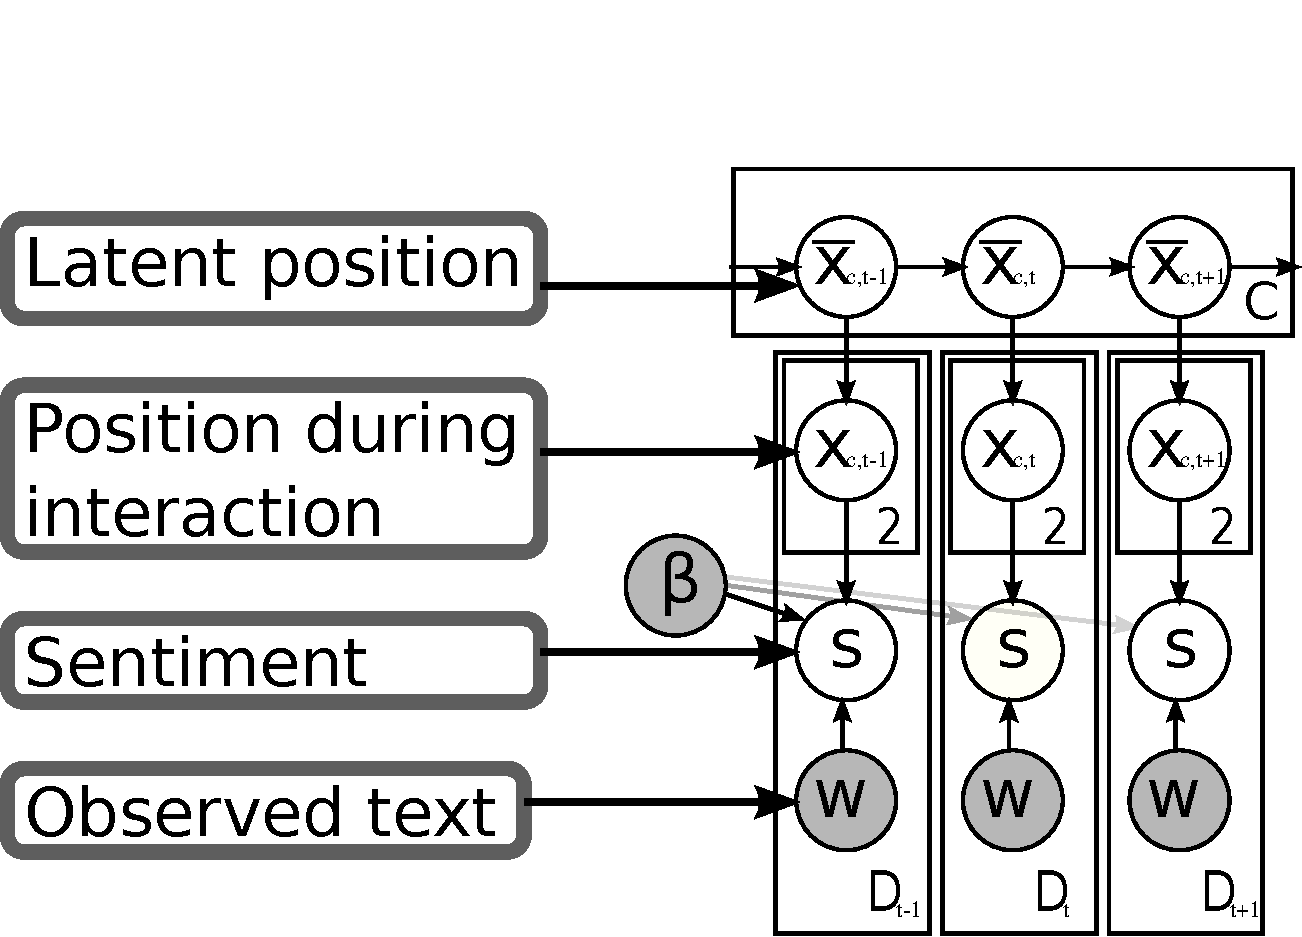
\includegraphics[width=0.8\textwidth]{figs/countries_gm_norev.pdf}
  \end{center}
}

% \frame {
%   \frametitle{The relationship between countries over time}
%   \begin{center}
%     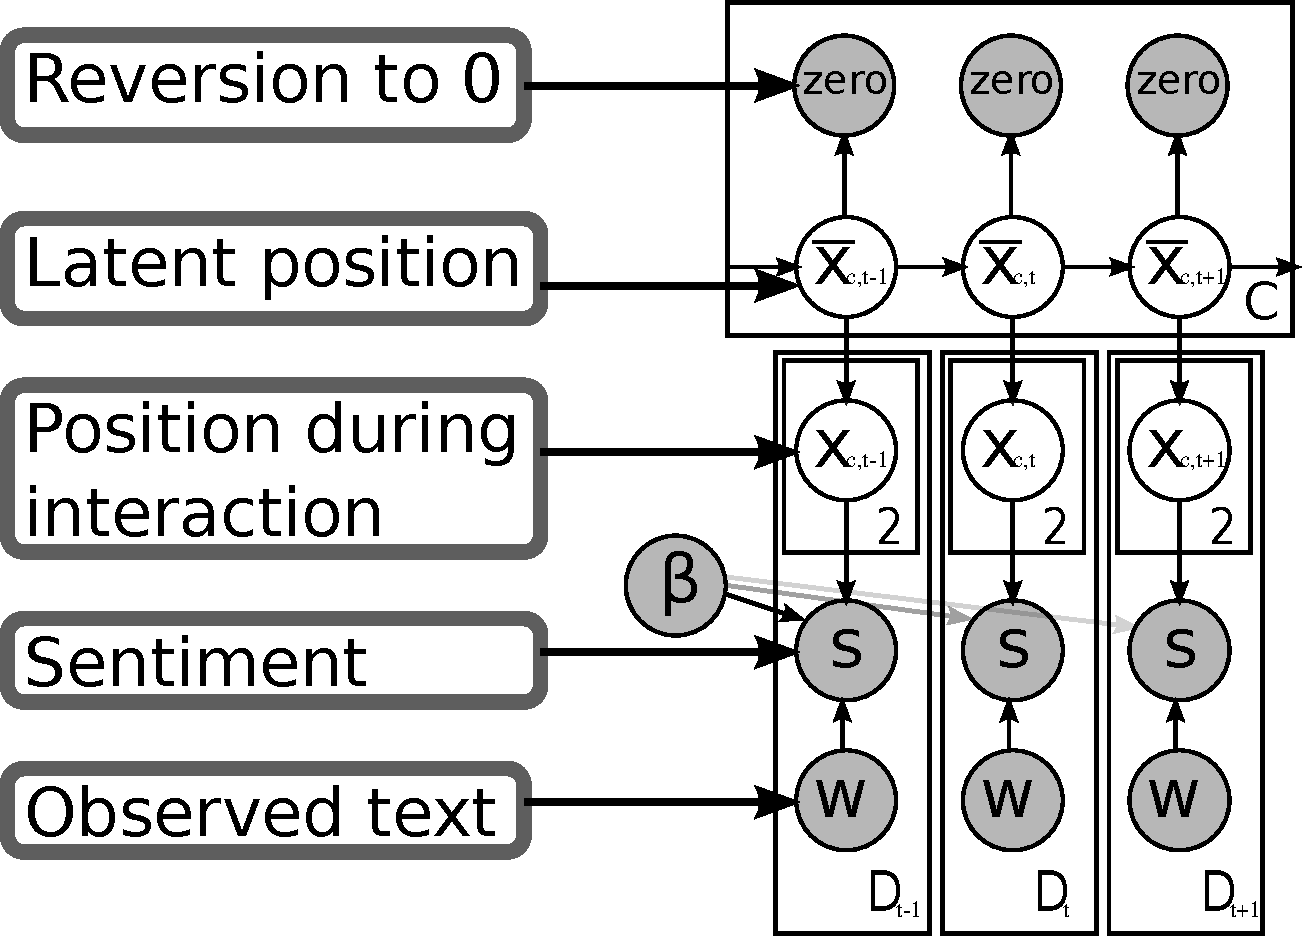
\includegraphics[width=0.8\textwidth]{figs/countries_gm.pdf}
%   \end{center}
% }

% \frame {
%   \frametitle{Labeling sentiment}
%   \center
%   
\includegraphics{figs/amazon_mechanical_turk.jpg}
%   \begin{enumerate}
%   \item We found all pairs of paragraphs from the New York Times which
%     discussed exactly two countries
%   \item A random sample of 3607 paragraphs from \emph{New York Times} articles from 1988 to 2008 were labeled by Amazon Mechanical Turk workers
%   \item Raters rated news articles on the scale $-5, -3, -1, 1, 3, 5$
%   \end{enumerate}
% }

\frame {
 \frametitle{Experiments}
 \begin{itemize}
 \item Randomly select 3607 paragraphs discussing pairs of 245
   countries and territories. \\
  \item Label each of these paragraphs' sentiment. \\
  \item Fit sentiment model parameters $\beta$ on a set of training
    paragraphs. \\
  \item Fit the spatial sentiment model with these parameters on
    47,105 paragraphs from 1988 to 2008 (MAP estimation) \\
%  \item Evaluate model sentiment prediction on the heldout 244 test
%    paragraphs.
 \end{itemize}
}

%  \frame {
%   \frametitle{Analysis with this model}
%   To perform analysis with this model:
% %\begin{frame}[plain]
% %\makebox[\linewidth]{\rule{12cm}{3cm}}
% %\end{frame}
%   \begin{enumerate}
%     \item Fit the posterior (we used MAP)
%     \item Inspect countries' means $\bar x_{c, \cdot}$
%     \item Inspect the relationship between countries' means $\bar x_{c_1, t} \bar x_{c_2, t}$

%   \end{enumerate}
%  }


\frame {
 \frametitle{Results: countries' latent positions}
 Countries' positions by the \emph{intercept / distance} link function \\
\center $\mathcal{F}(\bm x_1, \bm x_2) = y_1 + y_2 - \log(|| \bm z_{1} - \bm
 z_{2} ||_2^2 + 1)$ \\
 \center 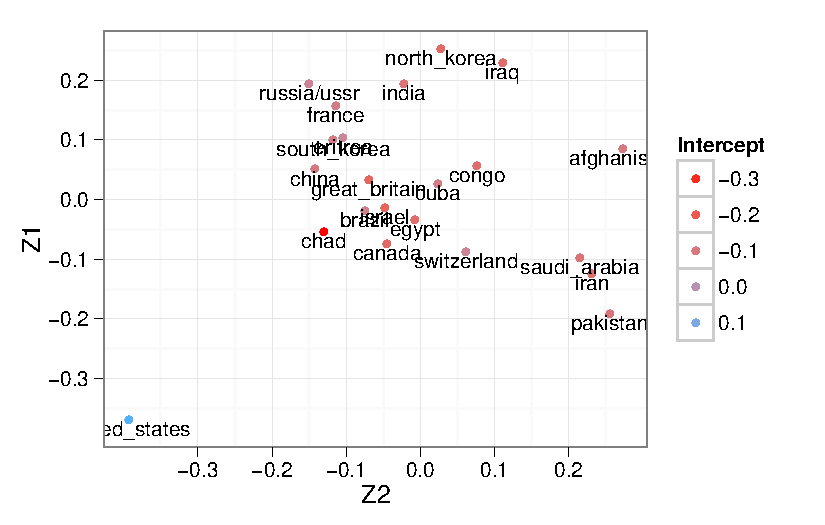
\includegraphics[width=1.0\textwidth]{figs/011_static_positions_mturk.pdf} \\
%    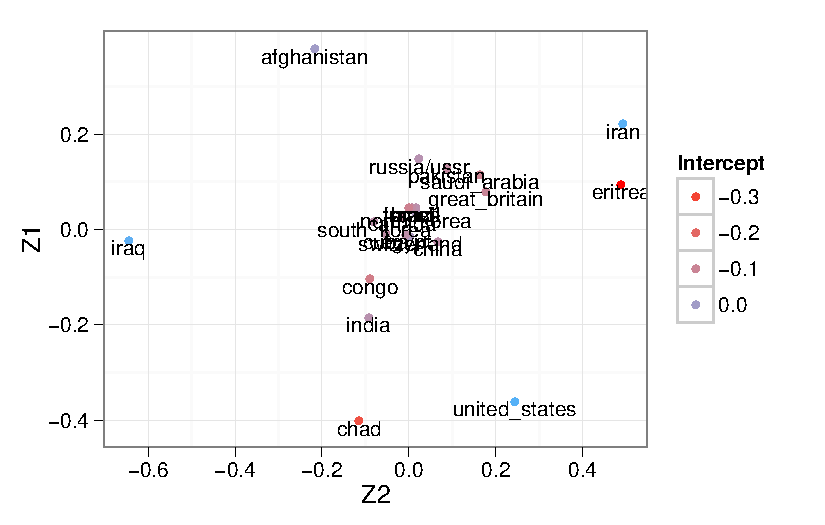
\includegraphics[width=0.5\textwidth]{figs/011_static_positions_cow.pdf}
    \center
    \Large Mechanical Turk \\
}

% \frame {
%  \frametitle{Results: selected countries' mutual sentiment with the U.S.}
%  \begin{center}
%  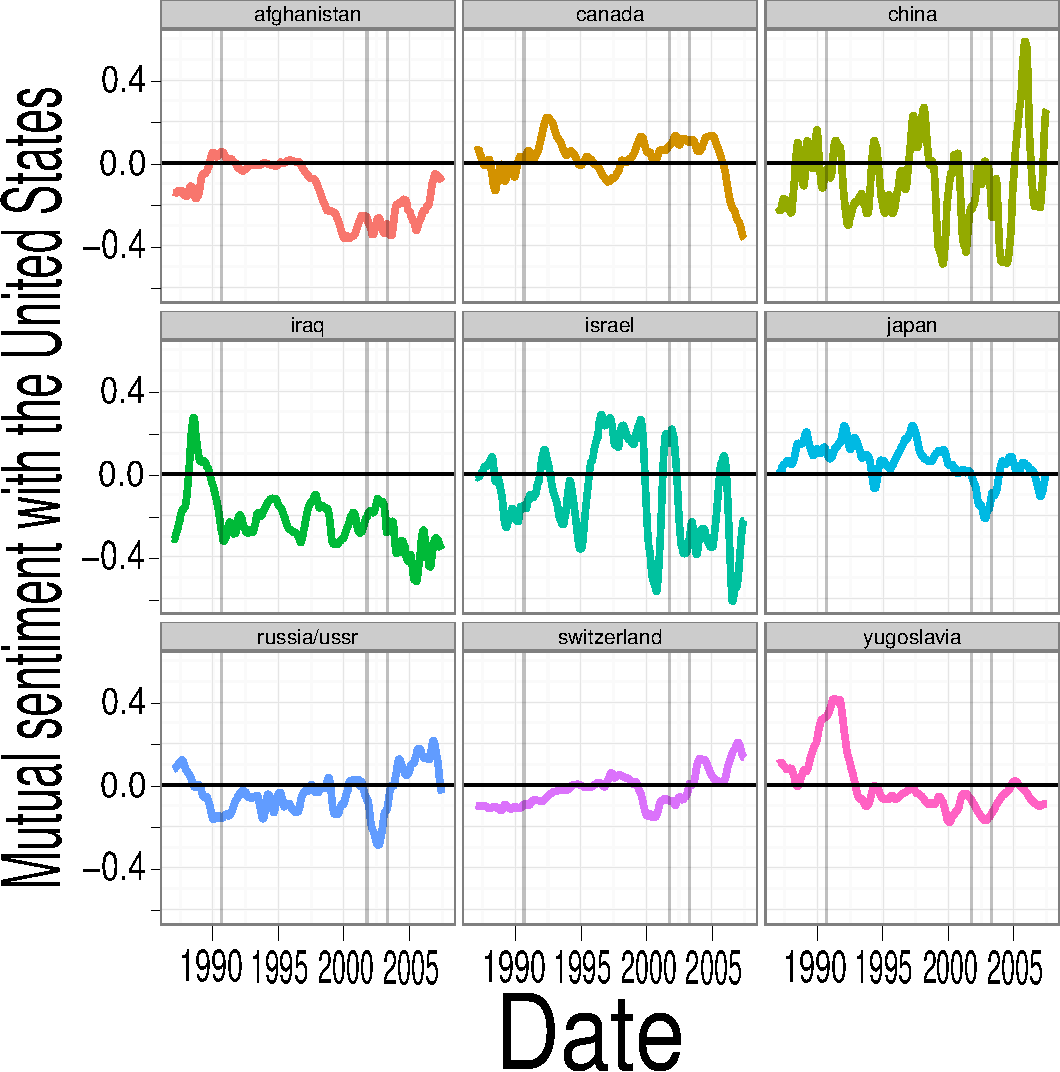
\includegraphics[height=0.8\textwidth]{figs/002_us_vs_everyone.pdf}
%  \end{center}
% }

% \frame {
%  \frametitle{Results: selected countries' mutual sentiment with Spain}
%  \begin{center}
%  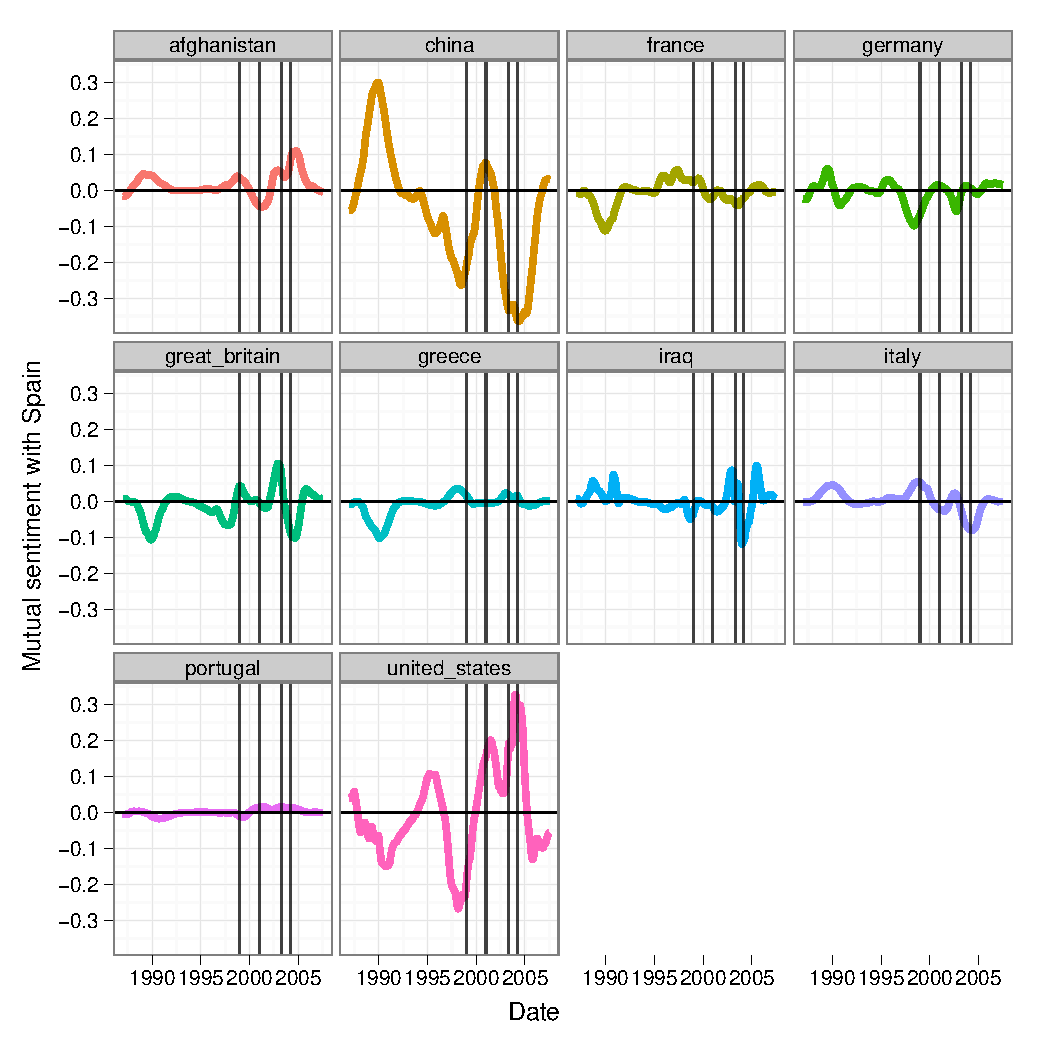
\includegraphics[height=0.8\textwidth]{figs/002_spain_vs_everyone.pdf}
%  \end{center}
% }

\frame {
  \frametitle{Results: evaluation}
  \begin{itemize}
    \item We measured the model's ability to predict text sentiment
      $\bm \beta^T \bm w_d$. \\
    \item The \emph{inner product / intercept} model is consistently
      the best model. \\
      \begin{itemize}
        \item Without an intercept, \emph{inner product} performs
          poorly. \\
        \item \emph{distance / intercept} performs well without time,
          but it overfits when we model time. \\
      \end{itemize}
      \item The best dimension is about 5. \\
      \item The distances inferred using Mechanical Turk labels are
        very similar to Correlates of War distances. \\
      \item Experiments with unsupervised sentiment detection yielded
        an economics / military sentiment topic. \\
    \end{itemize}
}

\frame {
  \frametitle{Results: countries' positions over time}
\begin{figure}
  \center
    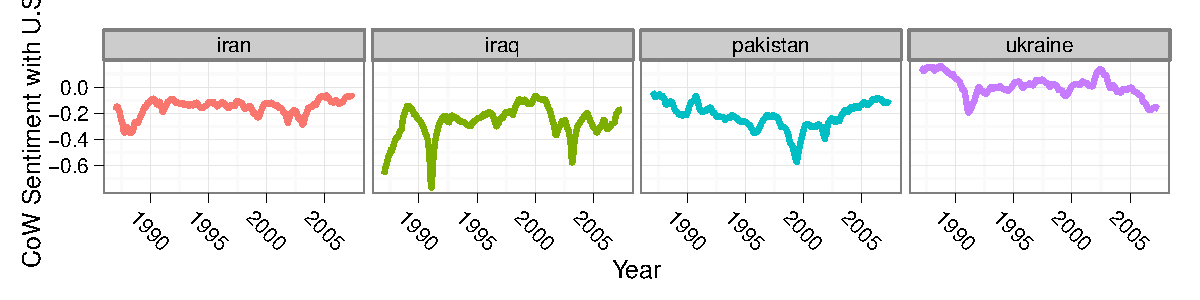
\includegraphics[width=1.1\textwidth]{figs/012_fr_cow_mutual_sentiment_with_us.pdf}
    \\
    \vspace{25pt}
    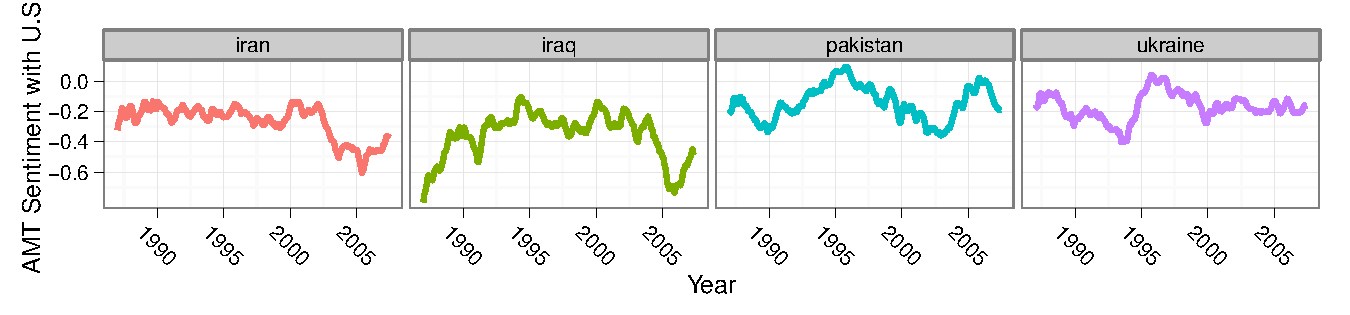
\includegraphics[width=1.1\textwidth]{figs/012_fr_mturk_mutual_sentiment_with_us.pdf}
  \label{fig:nation_positions_over_time}
\end{figure}
}

\frame {
  \frametitle{Finding influential documents in text corpora}
  \begin{itemize}
  \item Which of these articles were the most ``influential''?
  \item We can again use the text of documents to answer this question.
    \begin{enumerate}
    \item Make the idea of ``ideas changing through time'' explicit.
      \tiny \textcolor{gray}{\cite{blei:2006}}
      \normalsize
    \item Encode our assumptions about what it means to be
      ``influential''
      \tiny \textcolor{gray}{\cite{gerrish:2009}} \normalsize
    \item Infer the values of our ``influence'' metric from data.
    \begin{figure}
      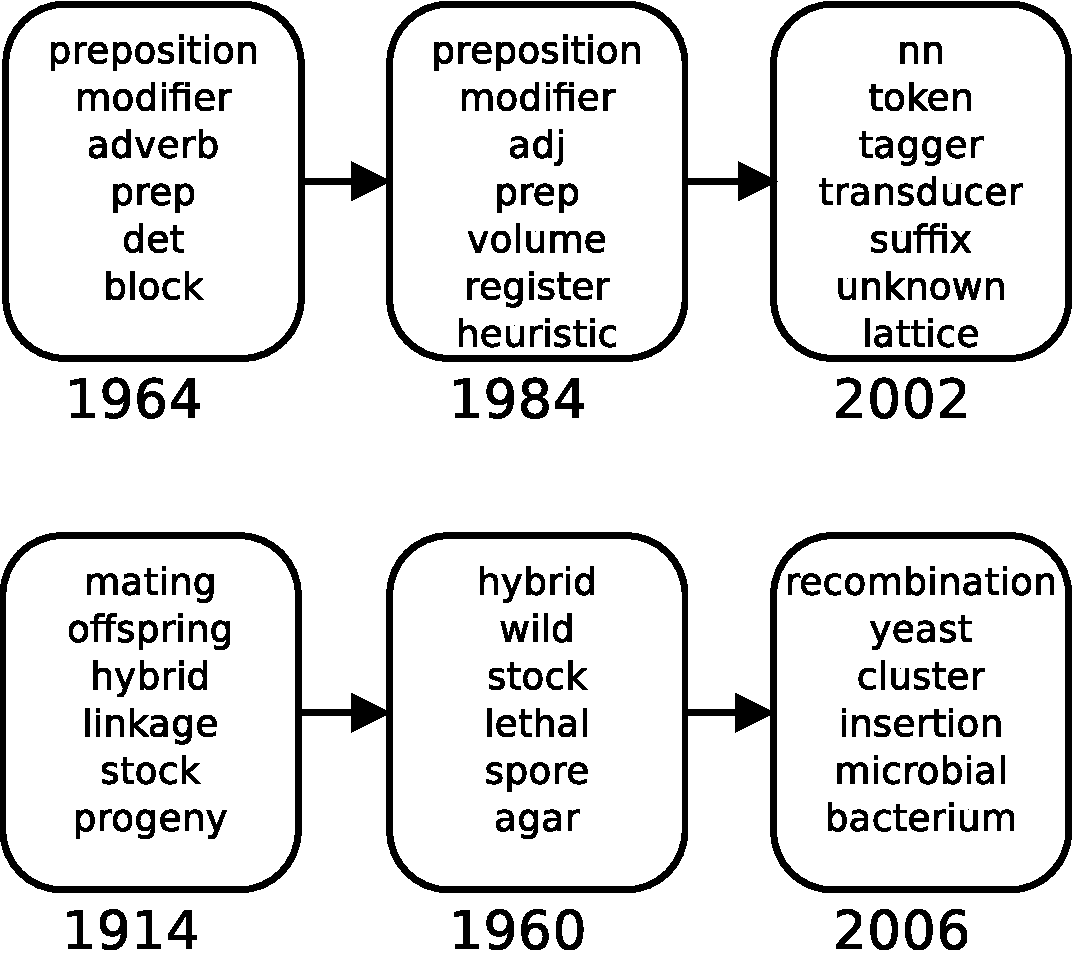
\includegraphics[width=0.4\textwidth]{figs/dynamic_topics.pdf}
    \end{figure}
    \end{enumerate}
  \end{itemize}
  \small
}

% \frame{
%   \frametitle{Current work and future directions}
%   \begin{itemize}
%   \item Sentiment intercepts for each country
%   \item Infer asymmetric relationships
%   \item Application to other dyads
%   \item Infer unsupervised relations
%     \begin{itemize}
%     \item Sentiment is only one dimension
%     \item Similar to relational topic models \cite{chang:2009}
%     \end{itemize}
%   \end{itemize}
% }


% \frame {
%  \frametitle{Predicting Legislative Votes}
%   \hspace{155pt}
%   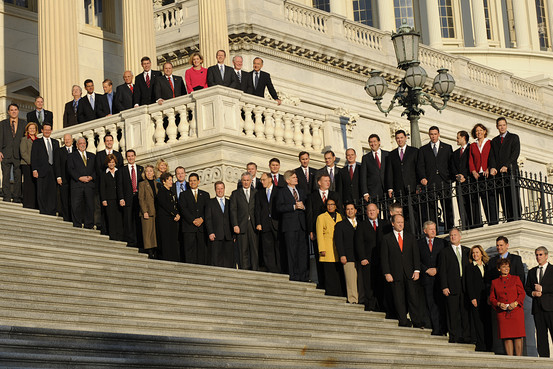
\includegraphics[width=0.34\textwidth]{figs/newcongress_photo_G_20090105182921.jpg}
%   \[
% 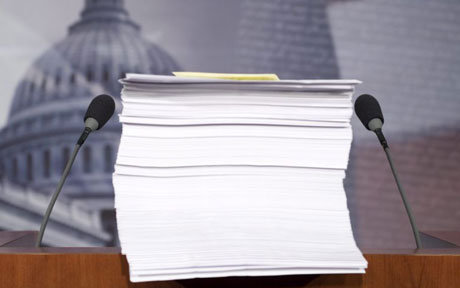
\includegraphics[width=0.34\textwidth,bb=30 110 450 230]{figs/health-bill.jpg}
%   \left[
%    \begin{array}{cccccccc}
%      \textcolor{black}{Y} & & & \textcolor{black}{N} & \textcolor{black}{Y} &  & & \textcolor{black}{Y} \\
%      & & & &                    &  & \textcolor{black}{N}  & \\
%      & & \textcolor{black}{Y} & & &  & & \\
%      \textcolor{black}{Y} & & & &                    & \textcolor{black}{N} &        & \textcolor{black}{N} \\
%      \textcolor{black}{N} & \textcolor{black}{N} & & & \textcolor{black}{Y} &  & & \textcolor{black}{Y} \\
%      & & & &                    &  &  & \textcolor{black}{N} \\
%      & & & & \textcolor{white}{Y} &  & \textcolor{white}{Y} & \\
%      \textcolor{white}{Y} & \textcolor{white}{Y} & & &                    &  & & \textcolor{white}{N} \\
%      & & \textcolor{white}{N} & \textcolor{white}{Y} &                    & \textcolor{white}{Y} & &  \\
%     \textcolor{white}{Y} & \textcolor{white}{N} & & & & & \textcolor{white}{Y} & \\
%    \end{array}
%    \right]
% \]
% \tiny 
% Images credit Susan Walsh (Associated Press) and EPA
% \normalsize
% }

% \frame {
%  \frametitle{Predicting Legislative Votes}
%   \hspace{155pt}
%   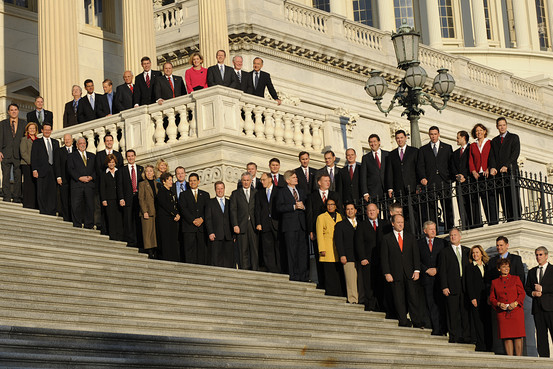
\includegraphics[width=0.34\textwidth]{figs/newcongress_photo_G_20090105182921.jpg}
%   \[
% 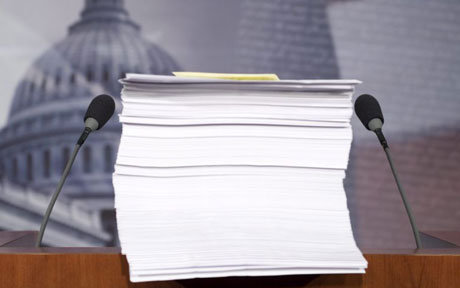
\includegraphics[width=0.34\textwidth,bb=30 110 450 230]{figs/health-bill.jpg}
%   \left[
%    \begin{array}{cccccccc}
%      \textcolor{black}{Y} & & & \textcolor{black}{N} & \textcolor{black}{Y} &  & & \textcolor{black}{Y} \\
%      & & & &                    &  & \textcolor{black}{N}  & \\
%      & & \textcolor{black}{Y} & & &  & & \\
%      \textcolor{black}{Y} & & & &                    & \textcolor{black}{N} &        & \textcolor{black}{N} \\
%      \textcolor{black}{N} & \textcolor{black}{N} & & & \textcolor{black}{Y} &  & & \textcolor{black}{Y} \\
%      & & & &                    &  &  & \textcolor{black}{N} \\
%      & & & & \textcolor{black}{Y} &  & \textcolor{black}{Y} & \\
%      \textcolor{white}{Y} & \textcolor{white}{Y} & & &                    &  & & \textcolor{white}{N} \\
%      & & \textcolor{white}{N} & \textcolor{white}{Y} &                    & \textcolor{white}{Y} & &  \\
%     \textcolor{white}{Y} & \textcolor{white}{N} & & & & & \textcolor{white}{Y} & \\
%    \end{array}
%    \right]
% \]
% \tiny 
% Images credit Susan Walsh (Associated Press) and EPA
% \normalsize
% }

% \frame {
%  \frametitle{Predicting Legislative Votes}
%   \hspace{155pt}
%   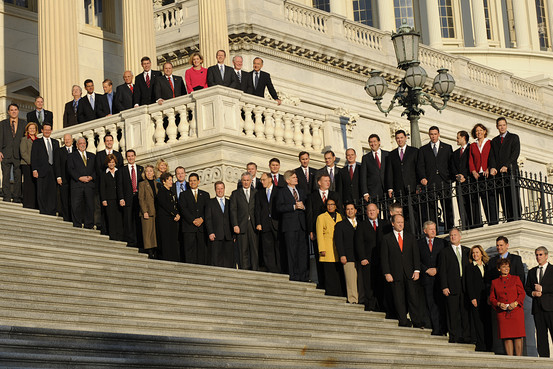
\includegraphics[width=0.34\textwidth]{figs/newcongress_photo_G_20090105182921.jpg}
%   \[
% 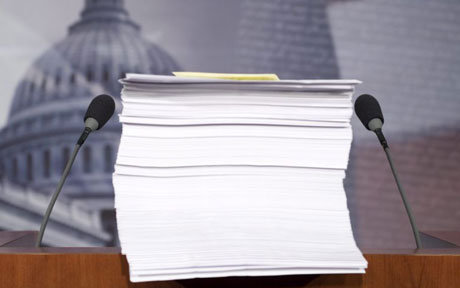
\includegraphics[width=0.34\textwidth,bb=30 110 450 230]{figs/health-bill.jpg}
%   \left[
%    \begin{array}{cccccccc}
%      \textcolor{black}{Y} & & & \textcolor{black}{N} & \textcolor{black}{Y} &  & & \textcolor{black}{Y} \\
%      & & & &                    &  & \textcolor{black}{N}  & \\
%      & & \textcolor{black}{Y} & & &  & & \\
%      \textcolor{black}{Y} & & & &                    & \textcolor{black}{N} &        & \textcolor{black}{N} \\
%      \textcolor{black}{N} & \textcolor{black}{N} & & & \textcolor{black}{Y} &  & & \textcolor{black}{Y} \\
%      & & & &                    &  &  & \textcolor{black}{N} \\
%      & & & & \textcolor{black}{Y} &  & \textcolor{black}{Y} & \\
%      \textcolor{black}{Y} & \textcolor{black}{Y} & & &                    &  & & \textcolor{black}{N} \\
%      & & \textcolor{white}{N} & \textcolor{white}{Y} &                    & \textcolor{white}{Y} & &  \\
%     \textcolor{white}{Y} & \textcolor{white}{N} & & & & & \textcolor{white}{Y} & \\
%    \end{array}
%    \right]
% \]
% \tiny 
% Images credit Susan Walsh (Associated Press) and EPA
% \normalsize
% }

% \frame {
%   \large
%   ``The government... began seeking ideas from academic
%   social scientists and corporations for ways to automatically scan
%   the Internet... ``
%   % ``So far there have been only scattered examples of the potential of
%   % mining social media.''
  
%   \vspace{30pt}
%   \tiny
%   \hspace{80pt} ”Government Aims to Build a ‘Data Eye in the Sky’”. The New York Times. Feb 11, 2011
% }

\frame {
  \begin{center}
    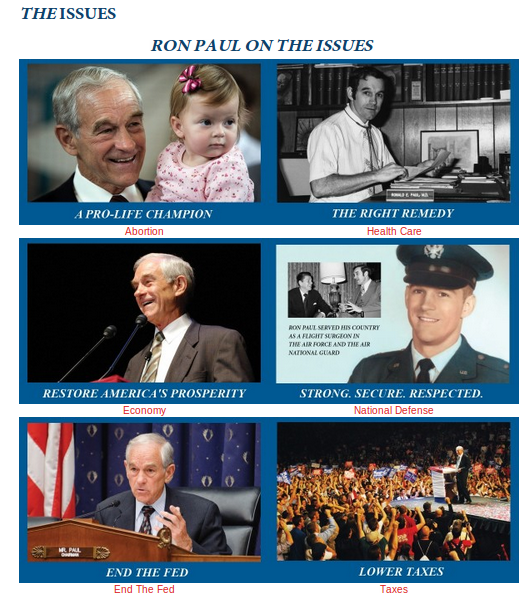
\includegraphics[height=0.9\textheight]{figs/ron_paul.png}
  \end{center}
}

\frame {
 \frametitle{Predicting Legislative Votes}
  \hspace{155pt}
  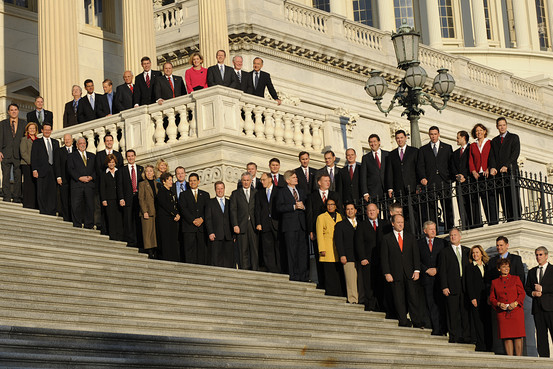
\includegraphics[width=0.34\textwidth]{figs/newcongress_photo_G_20090105182921.jpg}
  \[
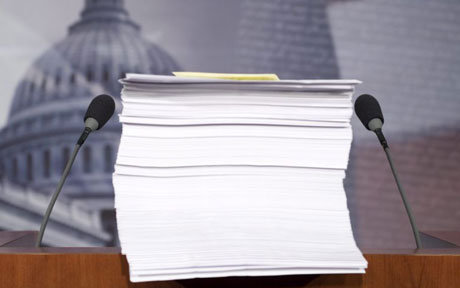
\includegraphics[width=0.34\textwidth,bb=30 110 450 230]{figs/health-bill.jpg}
  \left[
   \begin{array}{cccccccc}
     \textcolor{black}{Y} & & & \textcolor{black}{N} & \textcolor{black}{Y} &  & & \textcolor{black}{Y} \\
     & & & &                    &  & \textcolor{black}{N}  & \\
     & & \textcolor{black}{Y} & & &  & & \\
     \textcolor{black}{Y} & & & &                    & \textcolor{black}{N} &        & \textcolor{black}{N} \\
     \textcolor{black}{N} & \textcolor{black}{N} & & & \textcolor{black}{Y} &  & & \textcolor{black}{Y} \\
     & & & &                    &  &  & \textcolor{black}{N} \\
     & & & & \textcolor{black}{Y} &  & \textcolor{black}{Y} & \\
     \textcolor{black}{Y} & \textcolor{black}{Y} & & &                    &  & & \textcolor{black}{N} \\
     & & \textcolor{black}{N} & \textcolor{black}{Y} &                    & \textcolor{black}{Y} & &  \\
    \textcolor{white}{Y} & \textcolor{white}{N} & & & & & \textcolor{white}{Y} & \\
   \end{array}
   \right]
\]
\tiny 
Images credit Susan Walsh (Associated Press) and EPA
\normalsize
}

% \frame {
%  \frametitle{Predicting Legislative Votes}

%   \hspace{155pt}
%   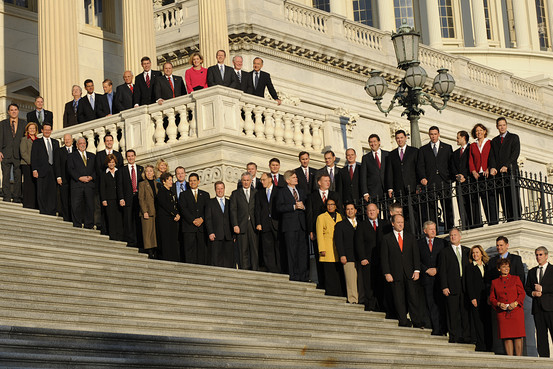
\includegraphics[width=0.34\textwidth]{figs/newcongress_photo_G_20090105182921.jpg}
%   \[
% 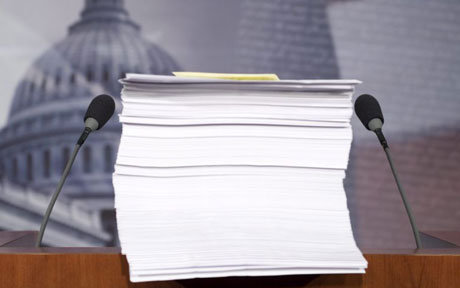
\includegraphics[width=0.34\textwidth,bb=30 110 450 230]{figs/health-bill.jpg}
%   \left[
%    \begin{array}{cccccccc}
%      \textcolor{black}{Y} & & & \textcolor{black}{N} & \textcolor{black}{Y} &  & & \textcolor{black}{Y} \\
%      & & & &                    &  & \textcolor{black}{N}  & \\
%      & & \textcolor{black}{Y} & & &  & & \\
%      \textcolor{black}{Y} & & & &                    & \textcolor{black}{N} &        & \textcolor{black}{N} \\
%      \textcolor{black}{N} & \textcolor{black}{N} & & & \textcolor{black}{Y} &  & & \textcolor{black}{Y} \\
%      & & & &                    &  &  & \textcolor{black}{N} \\
%      & & & & \textcolor{black}{Y} &  & \textcolor{black}{Y} & \\
%      \textcolor{black}{Y} & \textcolor{black}{Y} & & &                    &  & & \textcolor{black}{N} \\
%      & & \textcolor{black}{N} & \textcolor{black}{Y} &                    & \textcolor{black}{Y} & &  \\
%      \textcolor{blue}{?} & \textcolor{blue}{?} & & & & & \textcolor{blue}{?} & \\
%    \end{array}
%    \right]
% \]
% \tiny
% Images credit Susan Walsh (Associated Press) and EPA
% \normalsize
% }

% \frame{
%   \frametitle{Goal of this work}

%   We have two goals: \\
%   \begin{enumerate}
%     \item to predict votes on legislative text \\
%     \item to understand the issues driving these votes \\
%   \end{enumerate}

%   To achieve these goals, we will combine ideas from political science with machine learning: \\
%   \begin{itemize}
%     \item ideal point models \\
%     \item text regression and topic models \\
%   \end{itemize}
% }

% \frame{
%   \frametitle{Organization}
%   Introduce models \\

%   \begin{itemize}
%   \item Overview of a model to represent votes \\
%   \item Link from documents text to voting model parameters \\
%   \item Inference on these models \\
%   \end{itemize}

%   Experimental results \\
%   \begin{itemize}
%   \item Predictive performance \\
%   \item Text and political sentiment \\
%   \item Next steps and conclusions \\
%   \end{itemize}

% }

% \frame{
%   \frametitle{A model of voting patterns}
%   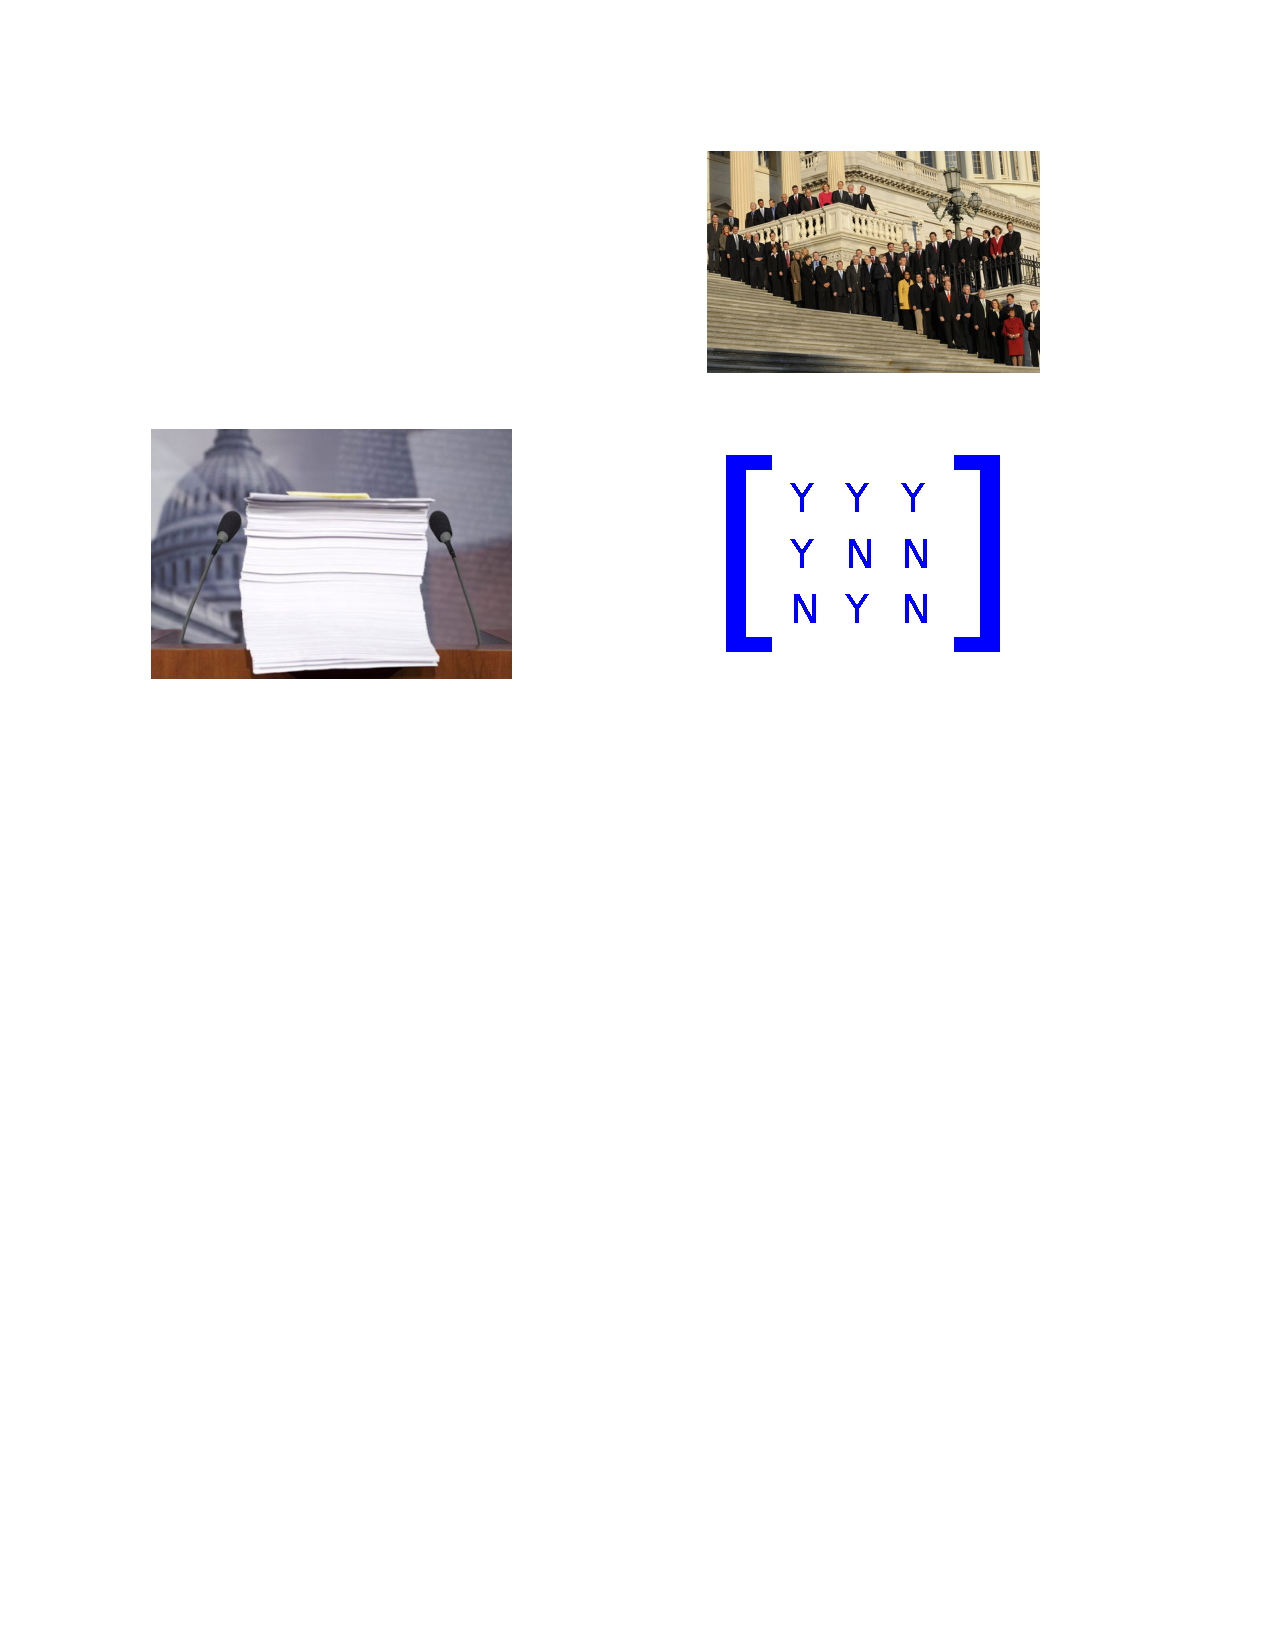
\includegraphics[width=1.0\textwidth]{figs/ideal_point_motivation_0.pdf}
% }

% \frame{
%   \frametitle{A model of voting patterns}
%   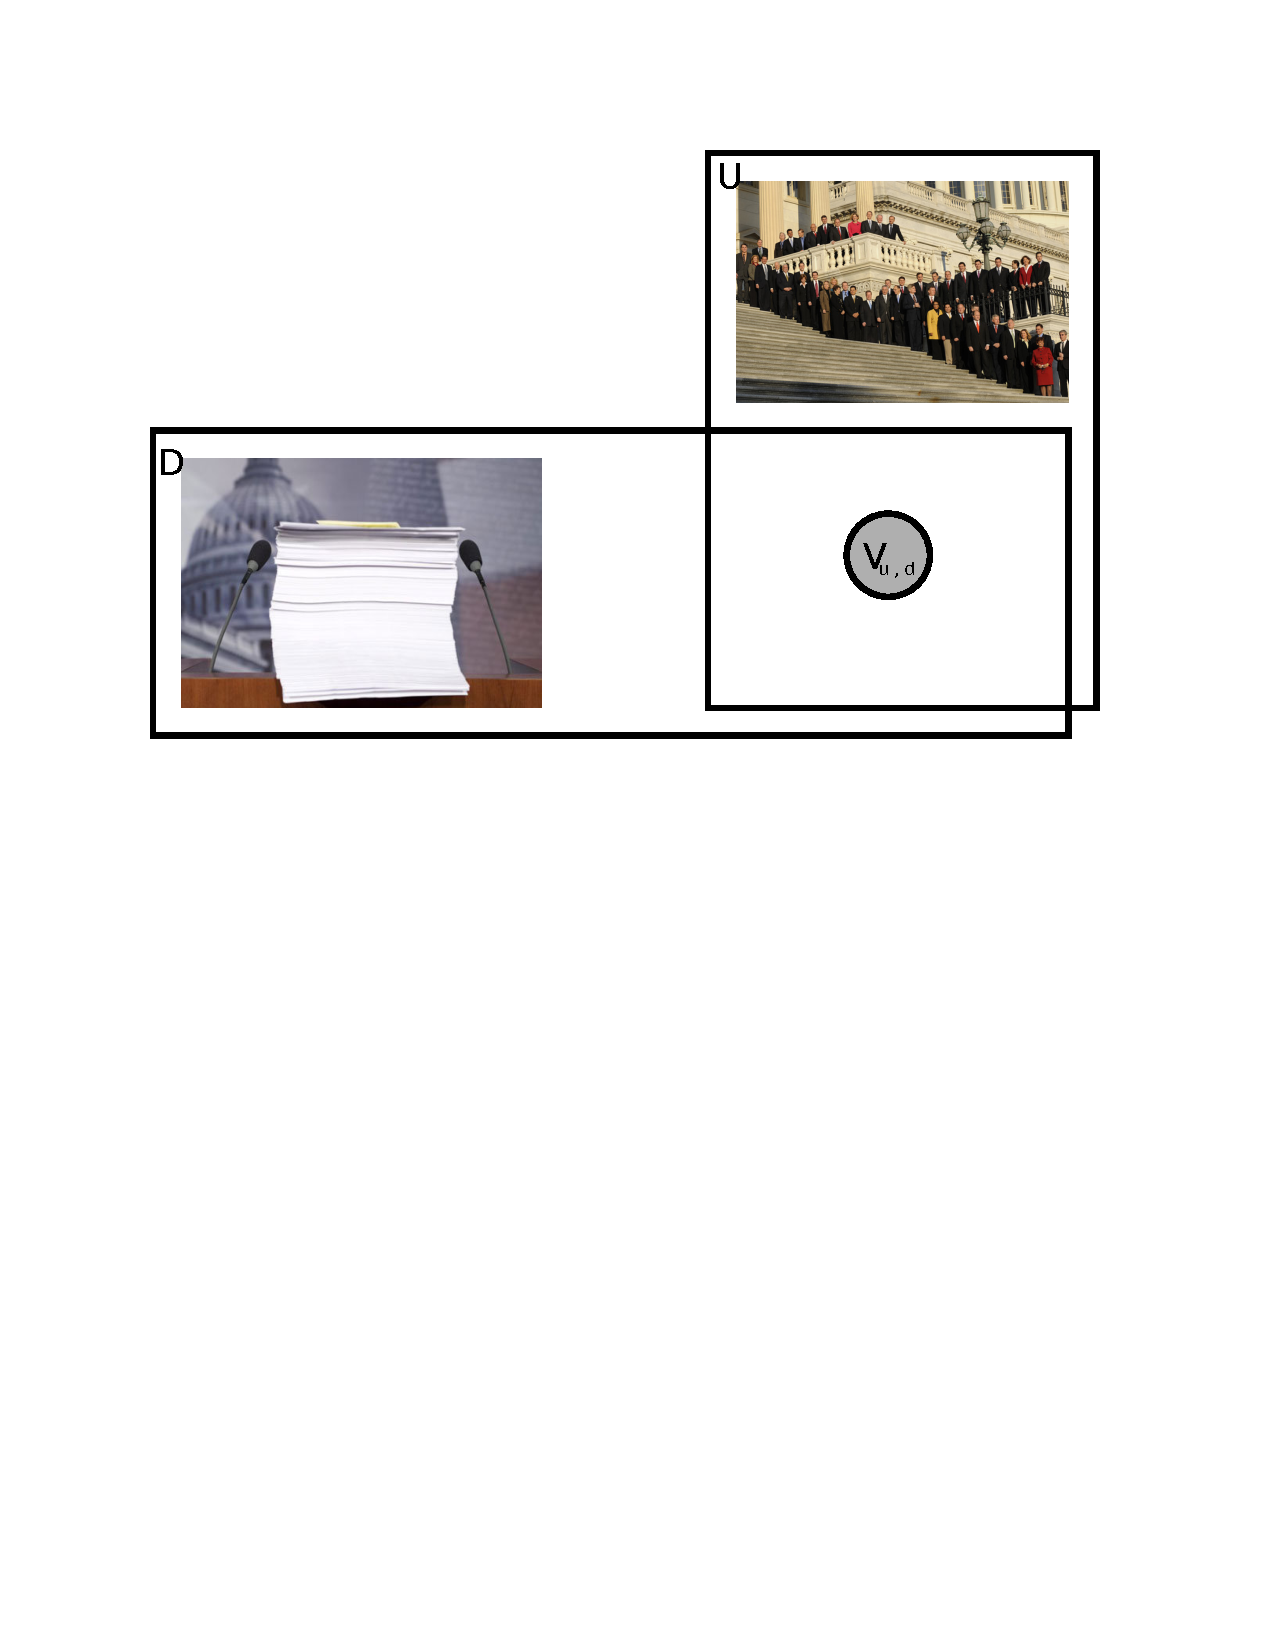
\includegraphics[width=1.0\textwidth]{figs/ideal_point_motivation_1.pdf} \\
% }

\frame{
  \frametitle{Item Response Theory}
  \tiny
    \textcolor{gray}{
  \begin{tabular}{lll}
Jackman, 2001 & Poole and Rosenthal, 1985 & Martin and Quinn, 2002 \\
Jounson and Albert, 1999 & Clinton et al., 2004 & \\
  \end{tabular}
}
  \large
%  \center
  \begin{align*}
    \vspace{-70pt}
    p(v_{ud} = \mbox{Yes}| x_u, a_d, b_d) = \mbox{logistic}(x_u \cdot a_d + b_d) \\
  \end{align*}
  \normalsize
  \vspace{20pt}
  \center
  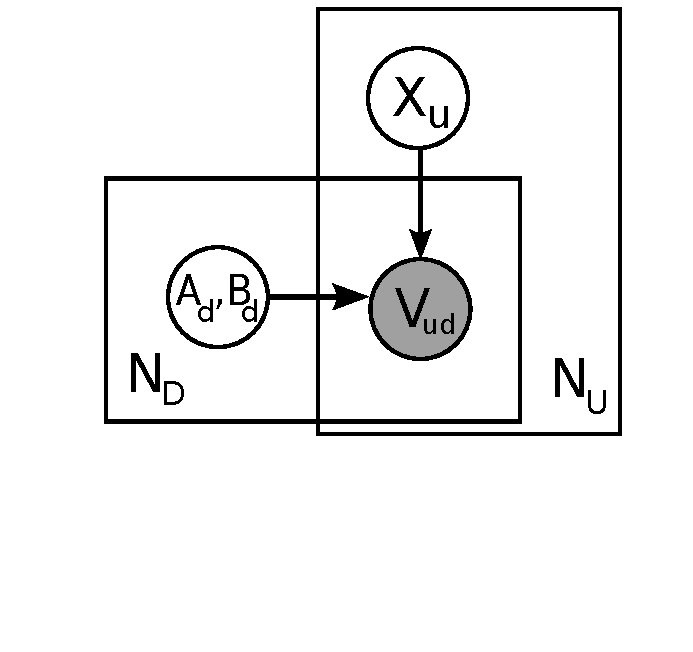
\includegraphics[width=0.6\textwidth]{figs/ip_gm.pdf} \\
}

\frame{
  \frametitle{Ideal points}
  Ideal points $\textcolor{blue}{x_u}$ position lawmakers in a latent political space.
  \tiny
    \textcolor{gray}{
  \begin{tabular}{lll}
Jackman, 2001 & Poole and Rosenthal, 1985 & Martin and Quinn, 2002 \\
Jounson and Albert, 1999 & Clinton et al., 2004 & \\
  \end{tabular}
}
  \large
  \begin{align*}
    \vspace{-70pt}
    p(v_{ud} = \mbox{Yes}| x_u, a_d, b_d) = \mbox{logistic}(x_u \cdot a_d + b_d) \\
  \end{align*}
\normalsize
\vspace{10pt}
  \begin{center}
  \normalsize
  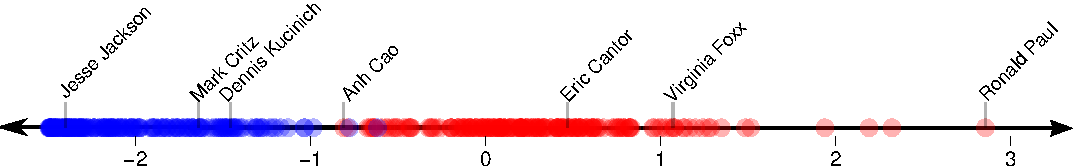
\includegraphics[scale=0.68]{figs/3393_example_ideal_points_final.pdf}
  \end{center}
\vspace{90pt}
}

% \frame{
%   \frametitle{Documents and ideal points}
%   \large
%   \[ p(v_{ud} = \mbox{Yes}| x_u, \textcolor{blue}{a_d}, \textcolor{blue}{b_d}) = \mbox{logistic}(x_u \cdot \textcolor{blue}{a_d} + \textcolor{blue}{b_d}) \]
%   \normalsize
% %  \begin{itemize}
% %    \item Discrimination $\textcolor{blue}{a_d}$ describes a bill's polarity
% %    \item Difficulty $\textcolor{blue}{b_d}$ describes a bill's overall popularity
% %    \item $ p(v_{i, j} = \mbox{Y}| x_u, \textcolor{blue}{a_d}, \textcolor{blue}{b_d}) = \mbox{logistic}(x_u \cdot \textcolor{blue}{a_d} + \textcolor{blue}{b_d})$
% %  \end{itemize}
%   \hspace{-20pt}
%   \vspace{-20pt}
%     \begin{tabular}{rll}
%   \onslide<1->{
%     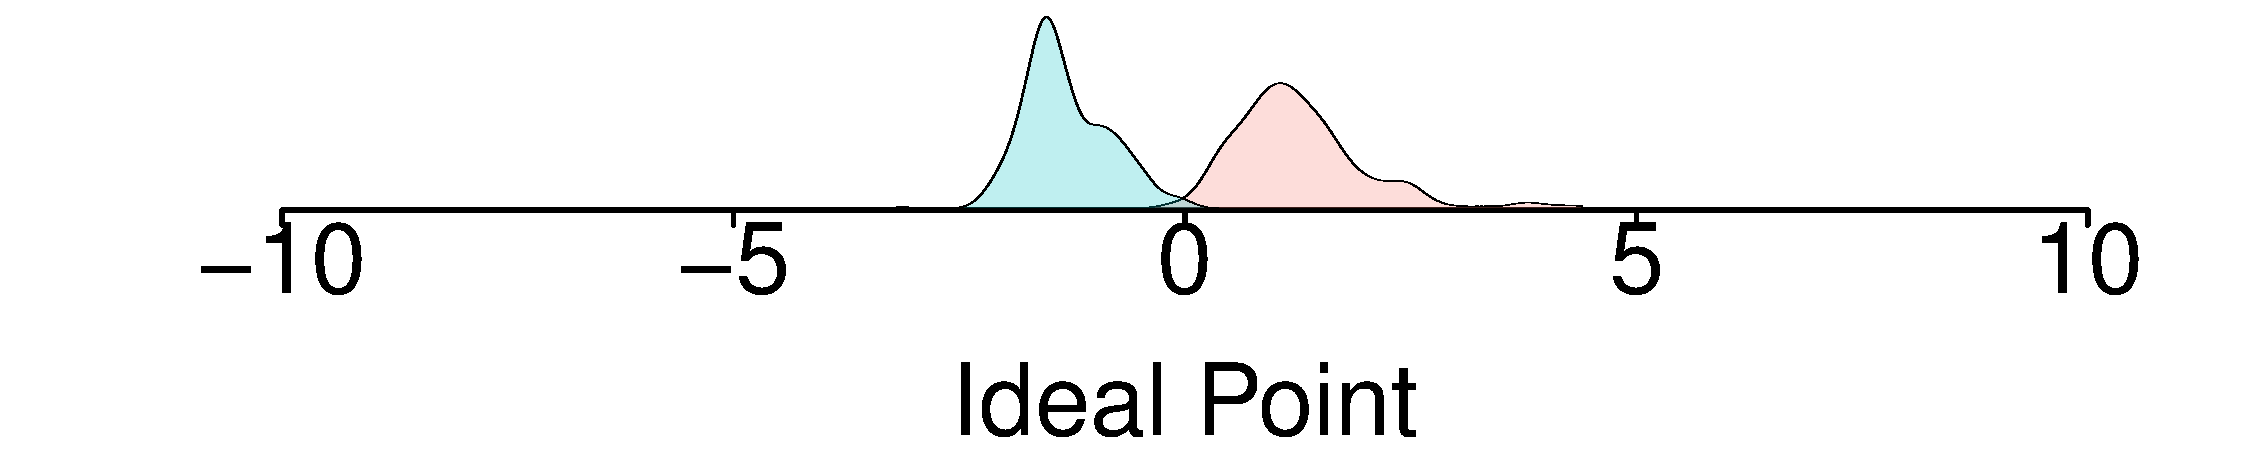
\includegraphics[width=0.7\textwidth]{figs/logistic_intro.pdf} &
%     $\textcolor{white}{a_d=1}$ & $\textcolor{white}{b_d=0}$ \\
%   }\newline
%   \vspace{5pt}
%   \onslide<1->{
%     
\includegraphics[width=0.7\textwidth]{figs/logistic_blank.pdf} &
%     $\textcolor{white}{a_d=20}$ & $\textcolor{white}{b_d=0}$ \\
%   }
%   \vspace{5pt}
%   \onslide<1->{
%     
\includegraphics[width=0.7\textwidth]{figs/logistic_blank.pdf} &
%     $\textcolor{white}{a_d=-0.4}$ & $\textcolor{white}{b_d=2}$ \\
%   }
%   \vspace{5pt}
%   \onslide<1->{
%     
\includegraphics[width=0.7\textwidth]{figs/logistic_blank.pdf} &
%     $\textcolor{white}{a_d=1}$ & $\textcolor{white}{b_d=-5}$ \\
%   }
%   \end{tabular}

% }

% \frame{
%   \frametitle{Documents and ideal points}
% %  \begin{itemize}
% %    \item Discrimination $\textcolor{blue}{a_d}$ describes a bill's polarity
% %    \item Difficulty $\textcolor{blue}{b_d}$ describes a bill's overall popularity
% %    \item
%   \large
%   \[ p(v_{ud} = \mbox{Yes}| x_u, \textcolor{blue}{a_d}, \textcolor{blue}{b_d}) = \mbox{logistic}(x_u \cdot \textcolor{blue}{a_d} + \textcolor{blue}{b_d}) \]
%   \normalsize
% %  \end{itemize}
%   \hspace{-20pt}
%   \vspace{-20pt}
%     \begin{tabular}{rll}
%   \onslide<1->{
%     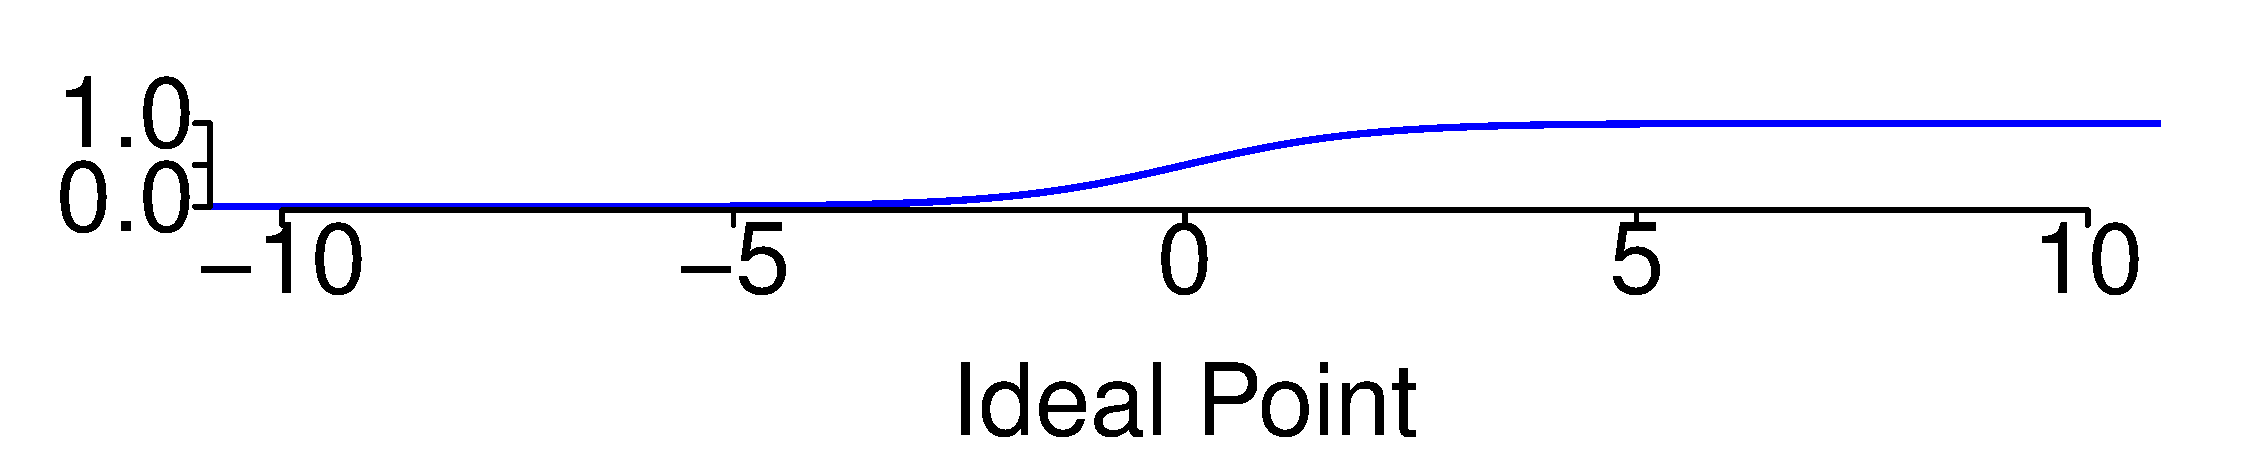
\includegraphics[width=0.7\textwidth]{figs/logistic_1_0.pdf} &
%     $a_d=1$ & $b_d=0$ \\
%   }\newline
%   \vspace{5pt}
%   \onslide<1->{
%     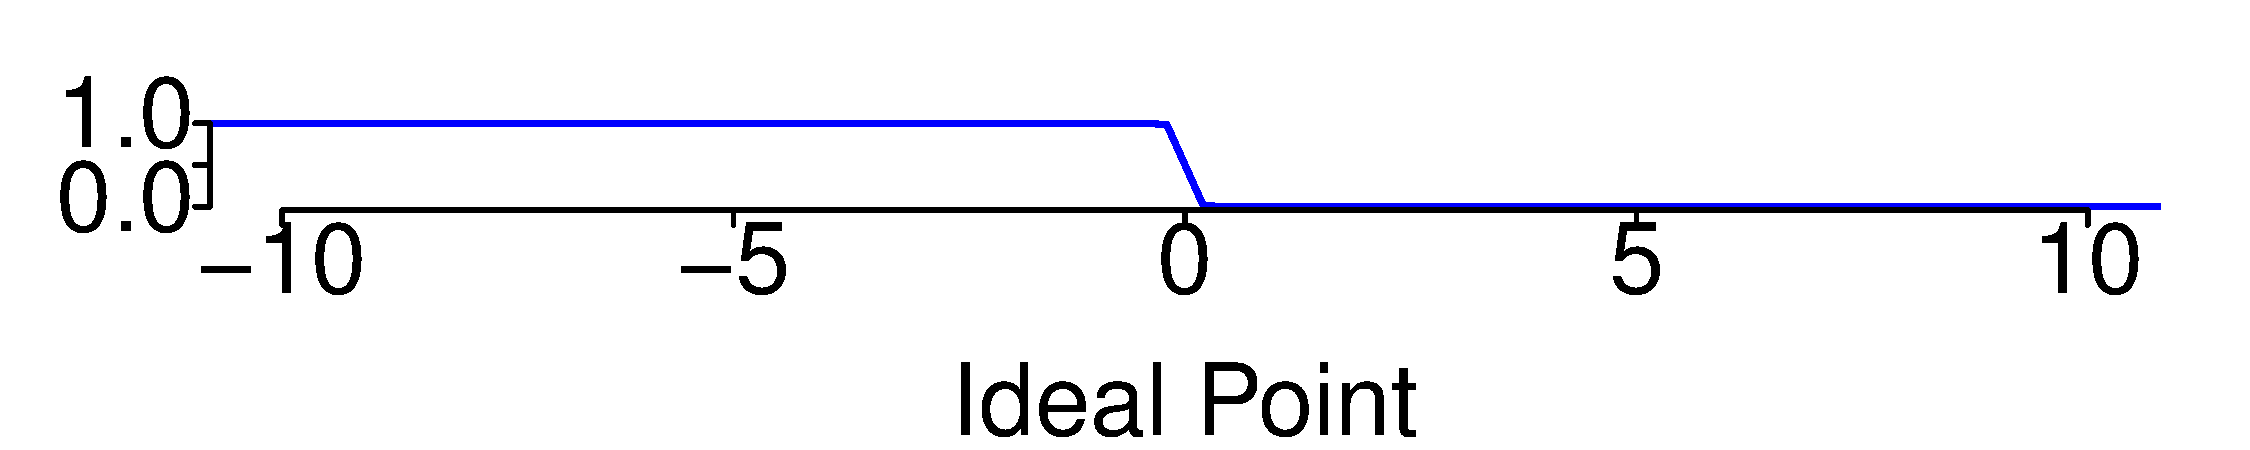
\includegraphics[width=0.7\textwidth]{figs/logistic_n20_0.pdf} &
%     $a_d=-20$ & $b_d=0$ \\
%   }
%   \vspace{5pt}
%   \onslide<1->{
%     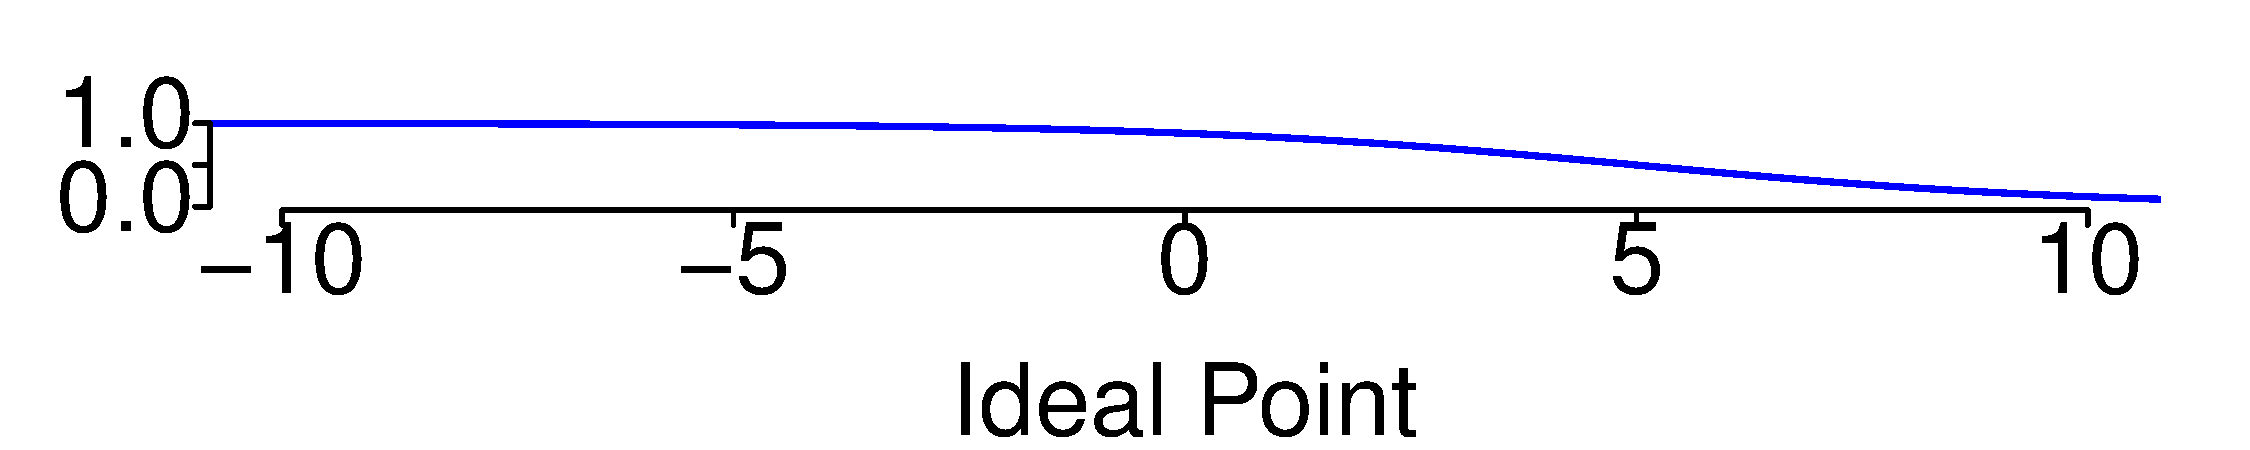
\includegraphics[width=0.7\textwidth]{figs/logistic_np4_2.pdf} &
%     $a_d=-0.4$ & $b_d=2$ \\
%   }
%   \vspace{5pt}
%   \onslide<1->{
%     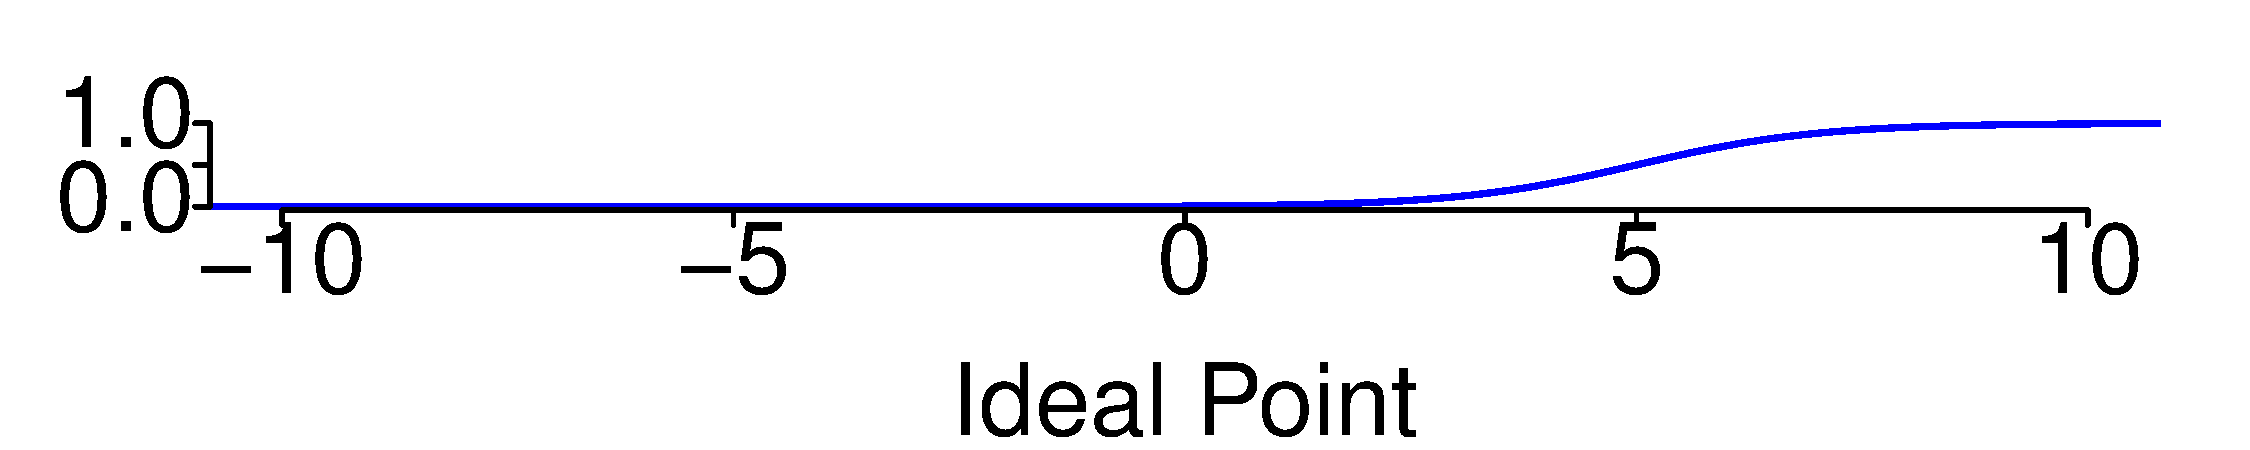
\includegraphics[width=0.7\textwidth]{figs/logistic_1_n5.pdf} &
%     $a_d=1$ & $b_d=-5$ \\
%   }
%   \end{tabular}
% }

% \frame{
%   \frametitle{Ideal points}
%   Ideal points $\textcolor{blue}{x_u}$ position lawmakers in a latent political space.
%   \tiny
%     \textcolor{gray}{
%   \begin{tabular}{lll}
% Jackman, 2001 & Poole and Rosenthal, 1985 & Martin and Quinn, 2002 \\
% Jounson and Albert, 1999 & Clinton et al., 2004 & \\
%   \end{tabular}
% }
% \normalsize
% \vspace{30pt}
%   \begin{center}
%   \normalsize
%   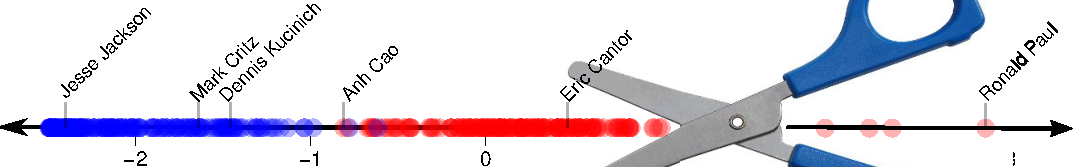
\includegraphics[scale=0.58]{figs/3393_example_ideal_points_cut1.pdf}
%   \end{center}
% \vspace{90pt}
% }

\frame{
  \frametitle{Ideal points}
  Ideal points $\textcolor{blue}{x_u}$ position lawmakers in a latent political space.
  \tiny
    \textcolor{gray}{
  \begin{tabular}{lll}
    \cite{jackman:2001} & \cite{poole:1985} & \cite{martin:2002} \\
    \cite{johnson:1999ch6} & \cite{clinton:2004} & \\
  \end{tabular}
}
  \large
  \begin{align*}
    \vspace{-70pt}
    p(v_{ud} = \mbox{Yes}| x_u, a_d, b_d) = \mbox{logistic}(x_u \cdot a_d + b_d) \\
  \end{align*}
\normalsize
\vspace{-5pt}
  \begin{center}
  \normalsize
  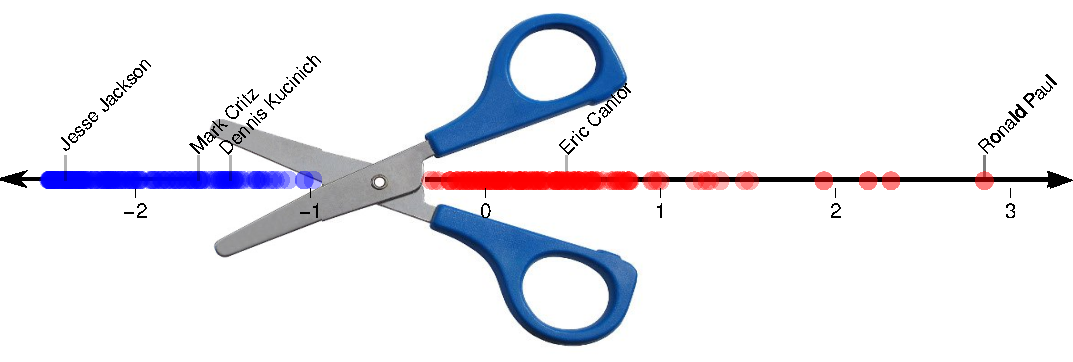
\includegraphics[scale=0.68]{figs/3393_example_ideal_points_cut2.pdf}
  \end{center}
  Each bill defines a \emph{cut point} that splits lawmakers.

\vspace{90pt}
}


% \frame{
%   \frametitle{Labeled Latent Dirichlet Allocation}
%   \small
%   \hspace{140pt} \textcolor{gray}{\cite{ramage:2009}} \\% \cite{ramage:2009} \\
%   \large
%   \begin{center}
%   \begin{tabular}{cc}
%     \hspace{-0pt} 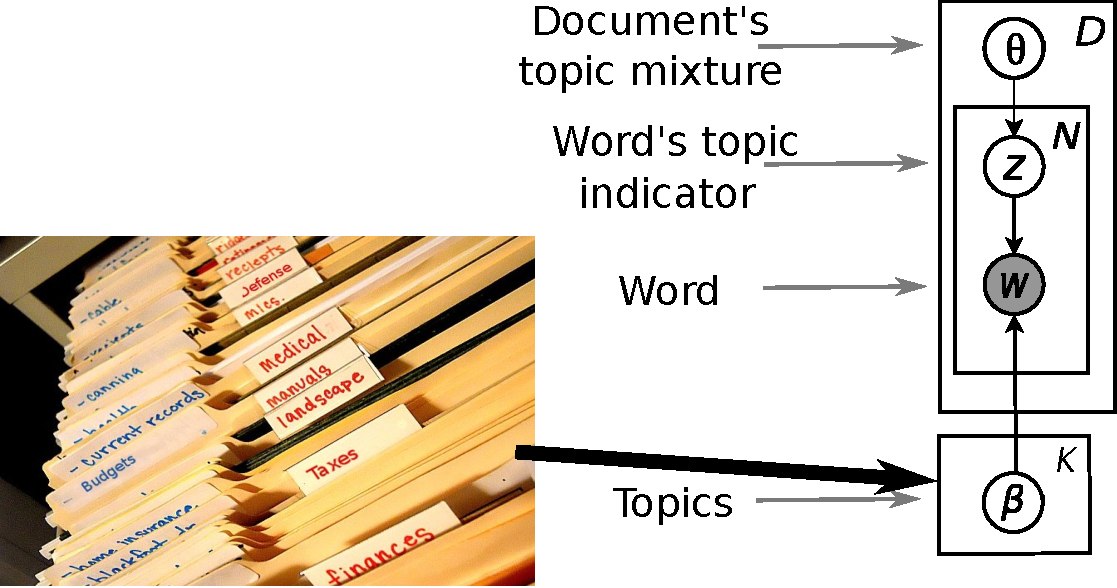
\includegraphics[width=0.85\textwidth]{figs/labeled_topics_gm.pdf}  \vspace{60pt} &
%   \end{tabular}
%   \end{center}
% }

\frame{
  \frametitle{Labeled Latent Dirichlet Allocation}
  \small
  \hspace{140pt} \textcolor{gray}{\cite{ramage:2009}} \\% \cite{ramage:2009} \\
  \large
  \begin{center}
  \begin{tabular}{cc}
    \hspace{-0pt} 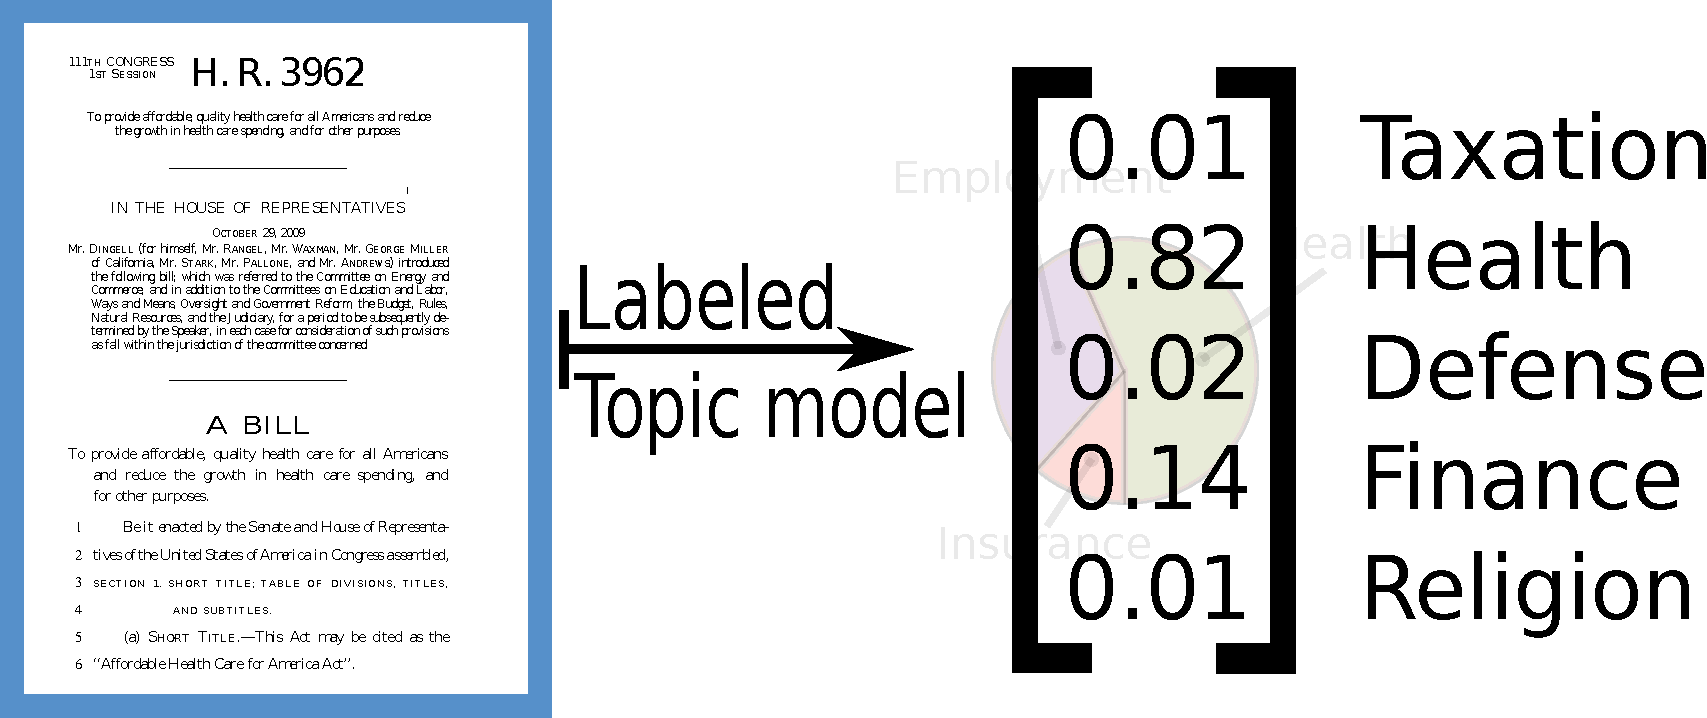
\includegraphics[width=0.85\textwidth]{figs/labeled_topics.pdf}  \vspace{60pt} &
%    \hspace{-40pt} 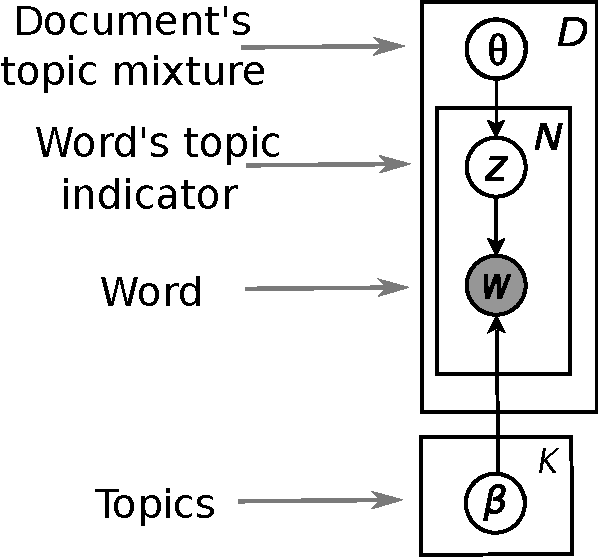
\includegraphics[width=0.55\textwidth]{figs/dtm.pdf}  \\
  \end{tabular}
  \end{center}
}

\frame{
  \frametitle{Labeled Latent Dirichlet Allocation - Example Topics}
  \vspace{8pt}
  \center
  \large
  \begin{tabular}{cccc}
    \textbf{Terrorism} & \textbf{Commemorations} & \textbf{Education}
    & \textbf{Transportation} \\
    \hline
    terrorist & nation & student & transportation \\
    york & serve & history & land \\
    September &  people & school & minor \\
    terrorist attack & percent & nation & nature \\
    attack &  life & university & minor \\
    Hezbollah & community & child & print \\
    nation & world & charter school & substitute \\
    national guard & family & college & tax \\
\end{tabular}

}

\frame{
  \frametitle{An issue-adjusted ideal point model}
  \tiny
    \textcolor{gray}{
%  \begin{tabular}{l}
%    Gerrish and Blei \\
%  \end{tabular}
}
  \large
%  \center
  \begin{align*}
    p(v_{ud} = \mbox{Yes}| \ldots) = \ldots
  \end{align*}
  \vspace{10pt}
  \begin{tabular}{c|c}
    $\mbox{logistic}(x_u \cdot a_d + b_d)$
 %   \vspace{30pt}
    &
    $\mbox{logistic}((x_u \textcolor{blue}{+ \bm z_u^T \theta_d}) \cdot a_d + b_d)$
%    \vspace{10pt}
    \\
    \begin{minipage}{2.3in}
      \vspace{40pt}
      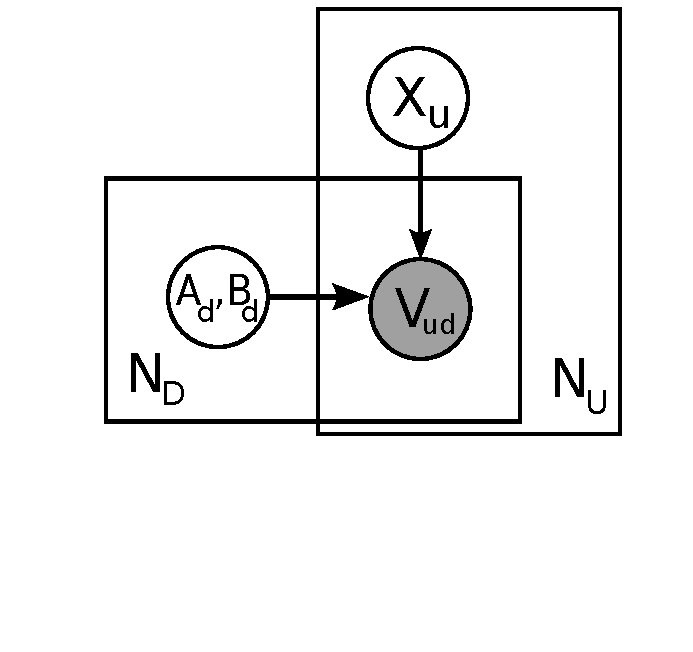
\includegraphics[width=0.98\textwidth]{figs/ip_gm.pdf} 
    \end{minipage}
      &
%      \vspace{30pt}
      \begin{minipage}{2.3in}
      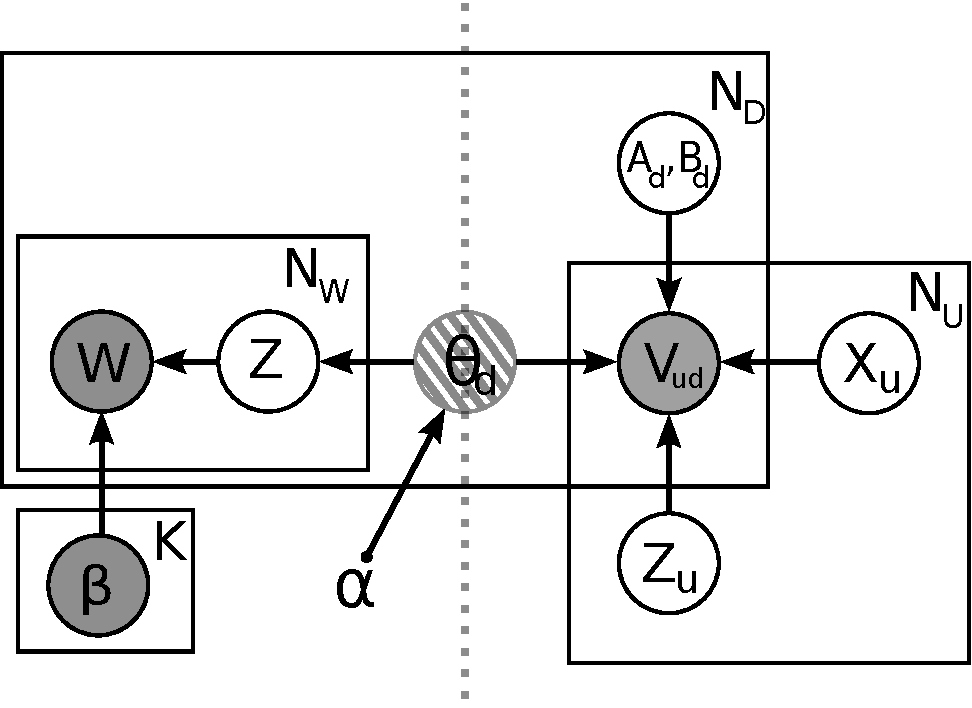
\includegraphics[width=0.98\textwidth]{figs/legis_gm.pdf}
      \end{minipage}
      \\
  \end{tabular}
  \normalsize
}


\frame {
  \frametitle{The U.S. House and Senate}
  \center
%  \begin{minipage}{2in}
    \center
    \textbf{The U.S. Senate} \\
  \center
\hspace{-14pt}
  \begin{tabular}{ccccc}
    \hline
    \hline
    \hspace{-8pt} \textbf{Congress} \hspace{-8pt} & \hspace{-8pt} {\textbf{Years}} \hspace{-8pt} & \textbf{Lawmakers} \hspace{-8pt} & \hspace{-4pt} \textbf{Bills} \hspace{-4pt} & \hspace{-4pt} \textbf{Votes} \\
    \hline
    106 & 1999-2000 & 81 & 101 & 7,612 \\
    107 & 2001-2002 & 78 & 76 & 5,547 \\
    108 & 2003-2004 & 101 & 83 & 7,830 \\
    109 & 2005-2006 & 102 & 74 & 7,071 \\
    110 & 2007-2008 & 103 & 97 & 9,019 \\
    111 & 2009-2010 & 110 & 62 & 5,936 \\
    \hline
  \end{tabular}
%  \end{minipage}
  \\
  \center
  \hspace{45pt}
\begin{minipage}{4.5in}
  \center
  \textbf{The House of Representatives} \\
  \vspace{-6pt}
  \center
  \begin{tabular}{ccccc}
    \hline
    \hline
    \hspace{-8pt} \textbf{Congress} \hspace{-8pt} & \hspace{-8pt} {\textbf{Years}} \hspace{-8pt} & \textbf{Lawmakers} \hspace{-8pt} & \hspace{-4pt} \textbf{Bills} \hspace{-4pt} & \hspace{-4pt} \textbf{Votes} \\
    \hline
    106 & 1999-2000 & 437 & 345 & 142,623 \\
    107 & 2001-2002 & 61 & 360 & 18,449 \\
    108 & 2003-2004 & 440 & 490 & 200,154 \\
    109 & 2005-2006 & 441 & 458 & 187,067 \\
    110 & 2007-2008 & 449 & 705 & 287,645 \\
    111 & 2009-2010 & 446 & 810 & 330,956 \\
    \hline
%  \end{tabular}
  \end{tabular}
  \end{minipage}
}

\frame {
  \frametitle{Posterior estimation - variational inference}
  \begin{itemize}
    \item As before, we only observe some data (votes and issue
      vectors). \\
      \vspace{10pt}
    \item We must estimate the posterior distribution $p(x_u, \bm
      z_u, a_d, b_d | \theta_d, v_{ud})$. \\
      \vspace{10pt}
    \item We used variational inference to do this. \\
      \vspace{10pt}
    \item Variational inference posits that the posterior can be
      described well by a simplified family of probability
      distributions (which is tractable). \\
      \vspace{10pt}
  \end{itemize}
}

\frame {
  \frametitle{Heldout log-likelihood}
  We used 6-fold cross-validation to assess the model.
  \center
  \begin{tabular}{|c|cccccc|}
    \hline
    \textbf{Model} & \multicolumn{6}{|c|}{\textbf{Senate}} \\
    \hline
    \textbf{Congress} & \hspace{-4pt} 106 \hspace{-5pt}
    & \hspace{-4pt} 107 \hspace{-5pt}
    & \hspace{-4pt} 108 \hspace{-5pt}
    & \hspace{-4pt} 109 \hspace{-5pt}
    & \hspace{-4pt} 110 \hspace{-5pt}
    & \hspace{-4pt} 111 \hspace{-4pt} \\
    \hline
    Ideal
    & \hspace{-4pt} -0.209 \hspace{-5pt}
    & \hspace{-4pt} -0.209 \hspace{-5pt}
    & \hspace{-4pt} -0.182 \hspace{-5pt}
    & \hspace{-4pt} -0.189 \hspace{-5pt}
    & \hspace{-4pt} -0.206 \hspace{-5pt}
    & \hspace{-4pt} -0.182 \hspace{-4pt} \\
    Issue
    & \hspace{-4pt} \textbf{-0.208} \hspace{-5pt}
    & \hspace{-4pt} \textbf{-0.209} \hspace{-5pt}
    & \hspace{-4pt} \textbf{-0.181} \hspace{-5pt}
    & \hspace{-4pt} \textbf{-0.188} \hspace{-5pt}
    & \hspace{-4pt} \textbf{-0.205} \hspace{-5pt}
    & \hspace{-4pt} \textbf{-0.180} \hspace{-4pt} \\
    \hspace{-5pt} Perm. Issue \hspace{-5pt}
    & \hspace{-4pt} -0.210 \hspace{-5pt}
    & \hspace{-4pt} -0.210 \hspace{-5pt}
    & \hspace{-4pt} -0.183 \hspace{-5pt}
    & \hspace{-4pt} -0.203 \hspace{-5pt}
    & \hspace{-4pt} -0.211 \hspace{-5pt}
    & \hspace{-4pt} -0.186 \hspace{-4pt} \\
    % Permuted Issue & & & & & & \\
    \hline
    \hline
    & \multicolumn{6}{|c|}{\textbf{House}} \\
    \hline
    Ideal & \hspace{-4pt} -0.168 \hspace{-5pt}
    & \hspace{-4pt} -0.154 \hspace{-5pt}
    & \hspace{-4pt} -0.096 \hspace{-5pt}
    & \hspace{-4pt} -0.120 \hspace{-5pt}
    & \hspace{-4pt} -0.090 \hspace{-5pt}
    & \hspace{-4pt} -0.182 \hspace{-4pt} \\
    Issue
    & \hspace{-4pt} \textbf{-0.166} \hspace{-5pt}
    & \hspace{-4pt} \textbf{-0.147} \hspace{-5pt}
    & \hspace{-4pt} \textbf{-0.093} \hspace{-5pt}
    & \hspace{-4pt} \textbf{-0.116} \hspace{-5pt}
    & \hspace{-4pt} \textbf{-0.087} \hspace{-5pt}
    & \hspace{-4pt} \textbf{-0.180} \hspace{-4pt} \\
    \hspace{-5pt} Perm. Issue \hspace{-5pt}
    & \hspace{-4pt} -0.210 \hspace{-5pt}
    & \hspace{-4pt} -0.211 \hspace{-5pt}
    & \hspace{-4pt} -0.100 \hspace{-5pt}
    & \hspace{-4pt} -0.123 \hspace{-5pt}
    & \hspace{-4pt} -0.098 \hspace{-5pt}
    & \hspace{-4pt} -0.187 \hspace{-4pt} \\
    \hline
  \end{tabular}
}

\frame{
  \frametitle{Issue-adjusted ideal points}
  \begin{center}
    $p(v_{ud} | x_u, \bm z_u^T, a_d, b_d) = \mbox{logistic}((x_u \textcolor{blue}{+ \bm z_u^T \theta_d}) \cdot a_d + b_d)$.
  \end{center}
  \tiny
    \textcolor{gray}{
%  \begin{tabular}{lll}
%Gerrish and Blei
%  \end{tabular}
}
\normalsize
\vspace{1pt}
  \begin{center}
  \normalsize
  \includegraphics[scale=0.65]{figs/3393_example_ideal_points_finance.pdf}
\vspace{10pt}
  \includegraphics[scale=0.65]{figs/3393_example_ideal_points_congressional_sessions.pdf} \\
  \end{center}
\vspace{90pt}
}

% \frame{
%   \frametitle{Adding text to the ideal point model}
%   \normalsize
%   We can use the text of legislation to infer bills' positions.
%   \large
%   \begin{eqnarray*}
%     \textcolor{white}{a_d \sim \mathcal{N}(\bm \eta_{\lambda}^T \bm w_d, \sigma^2)} \\
%     \textcolor{white}{b_d \sim \mathcal{N}(\bm \eta_{\kappa}^T \bm w_d, \sigma^2)} \\
%   \end{eqnarray*}
%   \normalsize
%   \vspace{-60pt}
%   \center
%   \includegraphics[width=1\textwidth]{figs/ideal_point_motivation_3.pdf}
%   \vspace{-20pt} \textcolor{white}{We regularize ${\bm \eta}$ using both ridge and lasso penalties.}
% }

% \frame{
%   \frametitle{Ideal Point Text Regression}
%   Regress document parameters on word counts:
%   \large
%   \begin{eqnarray*}
%     \lambda_d \sim \mathcal{N}(\bm \eta_{\lambda}^T \bm w_d, \sigma^2) \\
%     \kappa_d \sim \mathcal{N}(\bm \eta_{\kappa}^T \bm w_d, \sigma^2) \\
%   \end{eqnarray*}
%   \normalsize
%   \vspace{-60pt} 
%   \center
%   \includegraphics[width=1.0\textwidth]{figs/ideal_point_text_regression.pdf} \\
%   \vspace{-20pt} We regularize ${\bm \eta}$ using both ridge and lasso penalties.
% }

% \frame{
%   \frametitle{Ideal Point Topic modeling}
%   Use supervised topics to infer document parameters. \small \textcolor{gray}{Blei et al. 2008}
%   \large
%   \begin{eqnarray*}
%   \lambda_d \sim \mathcal{N}({\bm \eta_{\lambda}^T} \bar {\bm z_d}, \sigma^2) \\
%   \kappa_d \sim \mathcal{N}({\bm \eta_{\kappa}^T} \bar {\bm z_d}, \sigma^2) \\
%   \end{eqnarray*}
%   \normalsize
%   \vspace{-60pt}
%   \center
%   \includegraphics[width=0.74\textwidth]{figs/ideal_point_topic_model.pdf}
%   \vspace{-20pt} Topics adjust as regression parameters $\bm \eta$ are fit
% }

% \frame{
%   \frametitle{Experiments}
%   \begin{itemize}
%     \item We fit this model to each congressional session
%       (2-year period) from to Jan 1997 to Jan 2011. \\
%       \vspace{6pt}
%     \item Data is from Govtrack.us \\
%       \vspace{6pt}
%     \item There were: \\
%       \vspace{6pt}
%       \begin{itemize}
%       \item 4,447 bills \\
%       \vspace{6pt}
%       \item 1,269 lawmakers \\
%       \vspace{6pt}
%       \item 1,837,033 yea/nay roll-call votes \\
%     \end{itemize}  
%   \end{itemize}
% }

% % \frame{
% %   \begin{tabular}{c}
% %     \includegraphics[width=0.8\textwidth]{figs/health_care_ideal_point.pdf}
% %   \end{tabular}
% %   \begin{columns}
% %     \begin{column}{0.3\textwidth}
% % %      \setlength\fboxsep{4pt}
% % %      \setlength\fboxrule{0.5pt}
% % %    \fbox{\includegraphics[width=0.3\textwidth]{figs/111_ahcaa-1.pdf}}
% %     \fbox{\includegraphics[width=1.0\textwidth]{figs/111_ahcaa-1.pdf}}
% %     \end{column}
% %     \begin{column}{0.7\textwidth}
% %       \begin{itemize}
% %       \item 276 of 311 Democrats voted ``\textcolor{blue}{Yes}''.
% %       \item 217 of 217 Republicans voted ``\textcolor{red}{No}''.
% %         \vspace{20pt}
% %       \end{itemize}
% %     \end{column}
% %   \end{columns}
% % }

% \frame{
%   \begin{tabular}{c}
%     \includegraphics[width=0.8\textwidth]{figs/health_care_logistic.pdf} \\    
%   \end{tabular}
%   \begin{columns}
%     \begin{column}{0.3\textwidth}
% %      \setlength\fboxsep{4pt}
% %      \setlength\fboxrule{0.5pt}
% %    \fbox{\includegraphics[width=0.3\textwidth]{figs/111_ahcaa-1.pdf}}
%     \fbox{\includegraphics[width=1.0\textwidth]{figs/111_ahcaa-1.pdf}}
%     \end{column}
%     \begin{column}{0.7\textwidth}
%       \begin{itemize}
%       \item 276 of 311 Democrats voted ``\textcolor{blue}{Yes}''.
%       \item 276 of 276 Republicans voted ``\textcolor{red}{No}''.
%       \item Primary topic: \emph{care,applicable,coverage,hospital,eligible}
%       \item Inferred bill parameters are \\
%         \begin{center} $\lambda_d=1.5$, $\kappa_d=2.1$ \end{center}
%       \item Accuracy: 79\%
%       \item Baseline accuracy: 51\%
%       \end{itemize}
%     \end{column}
%   \end{columns}
% }


% \frame{
%   \frametitle{Results - Topics}
%   \center %\hspace{-30pt}
%   \begin{tabular}{|c|l|}
%     \hline
%     \textbf{Description} & \textbf{Topic summary \tiny (Example words)} \\
%     \hline
%     Popular & Military recognition
%   \tiny (\textcolor{blue}{weteran,war,serve,veterans,training,military}) \normalsize \\
%    (high $\bm \eta_{\kappa}$) & Recognition
%   \tiny (\textcolor{blue}{people, month, recognize, history, week, woman}) \normalsize \\
%   \hline
%   Unpopular & \textcolor{gray}{Anything polarizing} \\
%   \hline
%   Left-wing & Employment and eligibility
%   \tiny (\textcolor{blue}{eligible,credit,head,qualified,training}) \normalsize \\  
%   (low $\bm -\frac{\eta_{\kappa}}{\eta_{\lambda}}$) & Environmental policy
%   \tiny (\textcolor{blue}{energy,emission,epa,administrator,allowance}) \normalsize \\
%   & Regulation
%   \tiny (\textcolor{blue}{transfer,requires,contract,transportation,expense,corporation}) \normalsize \\
%   \hline
%   *Right-wing & Social Services
%   \tiny (\textcolor{blue}{medicare,social security act,clause,hospital}) \normalsize \\
%   (high $\bm -\frac{\eta_{\kappa}}{\eta_{\lambda}}$) & Land management
%   \tiny (\textcolor{blue}{land,subtitle,wilderness,river}) \normalsize \\
%   & Tobacco
%   \tiny (\textcolor{blue}{delivery, cigarette, tobacco, smokeless, sale, bills}) \normalsize \\
%   \hline
%   \end{tabular}
%   %     \end{itemize}
%   %   \item Liked by everyone (high $\bm \eta_{\kappa}$): \\
%   %     \begin{itemize}
%   %       \item Employment and eligibility: \textcolor{blue}{eligible, credit, head, } \\
%   %     \end{itemize}
%   %   \item Left-wing (low $\bm \eta_{\lambda}$): \\
%   %     \begin{itemize}
%   %     \item Environmental policy: \textcolor{blue}{energy,emission,epa,administrator,allowance,standard} \\
%   %     \item Regulation: \textcolor{blue}{transfer,requires,contract,transportation,expense,corporation}        \\
%   %     \item Procedural: \textcolor{blue}{eligible, subparagraph, credit, head, qualified} \\
%   %     \end{itemize}
%   %   \item Right-wing (high $\bm \eta_{\lambda}$) \\
%   %     \begin{itemize}
%   %        \item Social Services: \textcolor{blue}{medicare, social security act, clause, hospital} \\
%   %        \item Land Management: \textcolor{blue}{land, subtitle, wilderness, river, map, water} \\
%   %        \item Tobacco: \textcolor{blue}{delivery, cigarette, tobacco, smokeless, sale, bills} \\
%   %     \begin{itemize}
%   %   \end{itemize}
% }

% \frame{
%   \frametitle{Results - Prediction}
%   \begin{columns}
%     \begin{column}{0.6\textwidth}
%     \includegraphics[width=0.9\textwidth,height=1.1\textwidth]{figs/138_accuracy_by_session_topics_oral.pdf}
% %    \includegraphics[width=0.3 \textwidth]{figs/138_log_likelihood_by_session_topics_oral.pdf}
%   \end{column}
%   \begin{column}{0.5\textwidth}
%   \begin{itemize}
%     \item Predictive accuracy as high as 92\% with these models
%       \vspace{6pt}
%     \item Works best for 32-64 topics
%       \vspace{6pt}
%     \item Baseline ``assume everyone votes yes'' is black horizontal line
%     \item 93\% correct votes with a little more effort
%   \end{itemize}
%   \end{column}
%   \end{columns}
% }

% \frame{
%   \frametitle{Current and future directions}
%   Model ideal points over time, or with Kalman-type updates \\
%   \vspace{12pt}
%   Multiple ideal dimensions \\
%   \vspace{12pt}
%   Apply these models to other datasets: \\
%   \begin{itemize}
%     \item Content recommendation \\
%     \item Keyword-based advertising \\
%     \item Music recommendation \\
%   \end{itemize}
%   \vspace{12pt}
%   Use extra information: \\
%   \begin{itemize}
%     \item Transcripts of floor debates \\
%     \item Per-topic ideal points (uses more than 1 dimension) \\
%     \item Model ideal points over time \\
%   \end{itemize}  
% }

% \frame{
%   \frametitle{Summary}
%   The models we have discussed... \\
%   \begin{itemize}
%     \item Are predictive models for lawmakers' votes, \\
%       \vspace{6pt}
%     \item Include an exploratory model for discovering politicized topics 
%       and understanding the themes driving lawmakers, and \\
%       \vspace{6pt}
%     \item Have two key ideas at heart, \\
%       \vspace{6pt}
%       \begin{itemize}
%         \item Classic ideal point models \\
%             \vspace{6pt}
%         \item Supervision with text (e.g., topic models) \\
%       \end{itemize}
%       \vspace{6pt}
%     \item Can be used in a general collaborative filtering setting. \\
%   \end{itemize}
% }

% \frame{
%   \frametitle{Contact}
%   \begin{center}
%     \vspace{-120pt}  
%     \includegraphics[scale=0.58]{figs/134_interesting_senator_name_accuracy_by_ip_sample_all.pdf}
%   \end{center}
%   Contact
%   \begin{itemize}
%     \item Sean Gerrish (sgerrish@cs.princeton.edu)
%     \item David Blei (blei@cs.princeton.edu)
%   \end{itemize}
  
% }

\frame {
  \frametitle{Example: Ronald Paul}
  \begin{center}
  \includegraphics[height=0.9\textheight]{figs/3393_house_Ronald_Paul_400311.pdf}
  \end{center}
}

\frame {
  \frametitle{Example: Donald Young}
  \begin{center}
  \includegraphics[height=0.9\textheight]{figs/3393_house_Donald_Young_400440.pdf}
  \end{center}
}

\frame {
  \frametitle{Predicting votes on new bills}
  \begin{itemize}
    \vspace{-45pt}
    \item What if we have never seen votes on a bill before? \\
      \vspace{20pt}
    \item Remember, 
      $p(v_{ud} = \mbox{Yes} | ) = \mbox{logistic}(x_u a_d + b_d)$. \\
      \vspace{20pt}
    \item We cannot infer polarity $a_d$ and popularity $b_d$ from
      votes $\{ v_{ud} \}_d$. \\
      \vspace{20pt}
    \item We can predict $a_d$ and $b_d$ from the centent of bills.
      \tiny \textcolor{gray}{\cite{gerrish:2011}}
  \end{itemize}
}

\frame {
  \frametitle{Predicting votes on new bills: topic coefficients $a_d, b_d$}
  \includegraphics[width=1.06\textwidth]{figs/134_64_topic_plot.pdf}
}

\frame {
  \frametitle{Review}
  We discussed:
  \vspace{20pt}
  \begin{itemize}
  \item Latent-space models of foreign relations
  \item A method for discovering the issues driving lawmakers' votes
  \vspace{20pt}
  \item A method for discovering influential documents over time
  \item A way to predict lawmakers' votes on bills we have never seen
    before
  \item Stochastic optimization of the variational bound
  \end{itemize}
}

\frame {
  \frametitle{Funding}
  Funding
  \begin{itemize}
    \item National Science Foundation
    \item Office of Naval Research
    \item Yahoo! (CS department computers)
    \item Princeton Graduate School
    \item Facebook (travel)
    \item Google (travel)
    \end{itemize}
    % Advising and mentorship
    % \begin{itemize}
    % \item David Blei
    % \item Previous and current AI students
    % \end{itemize}
}


\section{Appendix}


\section*{Bibliography and Appendix}

\subsection*{Bibliography}

%\bibliographystyle{apalike}
\begin{frame}[allowframebreaks]
  \frametitle{Bibliography}  \tiny
  \bibliography{../bib} 
\end{frame}

\frame{
  \frametitle{Appendix}
}


% \frame {
%   \vspace{30pt}

% \vspace{5pt}
% \tiny \hspace{120pt} \textcolor{gray}{“The Age of Big Data.” The New York Times. Feb 11, 2012}
% \begin{center}
%   \includegraphics[width=1.1\textwidth,height=0.7\textheight]{figs/news.jpg} \\
% \end{center}
% }


% \subsection{The problem}

% \frame {
%  \frametitle{Identifying influential documents}

% %\begin{center}
% %\includegraphics[width=0.9\textwidth]{../figures/docs_basic.png} \newline
% %\end{center}
%  \begin{itemize}
%  \item Goal: Develop a measure of influence based only on language.
%  \item There are many specific application areas.
%    \begin{itemize}
%    \item News articles
%    \item Legal opinions
%    \item Scientific impact
%      %   \item Transcriptions of radio content and orations
%      \\
%    \end{itemize}
%  \item  Entire fields of study rely on work like this.
%    \begin{itemize}
%    \item History
%    \item Academic research
%    \item Much of Bibliometrics
%    \end{itemize}
%  \end{itemize}
% }

\frame {
  \frametitle{Common approach: citations}

  \begin{figure}
    \includegraphics[width=0.75\textwidth]{figs/citation_network.pdf}
  \end{figure}
  \begin{itemize}
    \item Traditionally, citations are used to identify influential documents.
    \item E.g.: \emph{A novel progressive spongiform encephalopathy in
      cattle}, \cite{wells:1987}
      (Cited by 709)
\vspace{2in}
  \end{itemize}
}

\frame {
  \frametitle{Common approach: citations}
  \begin{figure}
    \includegraphics[width=0.75\textwidth]{figs/no_citation_network.pdf}
  \end{figure}
  \begin{itemize}
    \item Citations are limited
      \begin{itemize}
      \item Hard to get
      \item May not exist
      \item Describe only one kind of influence
      \end{itemize}
    \item A language-based approach enables us to measure the influence of
      new kinds of documents
      \begin{itemize}
      \item News articles
      \item Historic manuscripts
      \end{itemize}
  \end{itemize}
}


%% \frame {
%%  \frametitle{Predicting influence in the absence of citations}
%%   \begin{figure}
%%     \includegraphics[width=0.8\textwidth]{../figures/topic_network.pdf}
%%   \end{figure}

%%   \begin{itemize}
%%     \item \label{def} Our \emph{intuition} is that influential
%%       documents change the language of their fields.
%%     \item Our \emph{goal} is to model the influence of documents
%%       without additional information.
%%   \end{itemize}
%%   Note that we assume documents influence their own subfields, not the
%% entire corpus.
%% \vspace{1in}
%% }


\frame {
  \frametitle{Methodology}
  \vspace{-.05in}
  \begin{centering}
    \begin{figure}
    \hspace{0in} \includegraphics[width=0.8\textwidth]{figs/influence_intuition.pdf} \newline
%    \begin{figure}
%      \includegraphics[width=0.4\textwidth]{../figures/docinf_gm.pdf}
%    \end{figure}
    \end{figure}
  \end{centering}
  \vspace{-.25in}
  \small
  \begin{itemize}
  \item The intuition: influential documents use language that becomes more popular in later years.
  \item We will encode these intuitions as assumptions in a
    probabilistic model to capture the interesting metrics.
    %    \item Build assumptions from \emph{topic models} into this model
  \item With posterior inference, we retrospectively see which documents have been influential on the corpus.
%  \item Related to \cite{leskovec:2009} and [Shaparenko et al., 2007], with a focus on topics.  
  \end{itemize}
  \normalsize
}


\frame{
  \frametitle{Latent Dirichlet Allocation}
  \small
  \hspace{140pt} \textcolor{gray}{\cite{blei:2003}} \\
  \normalsize Topic models decompose a corpus into a set of topics, i.e. distributions over terms.
  \large
  \center
  \begin{tabular}{cc}
    \hspace{-0pt} \includegraphics[width=0.55\textwidth]{figs/topics.pdf}  \vspace{60pt} &
    \hspace{-40pt} \includegraphics[width=0.55\textwidth]{figs/dtm.pdf}  \\
  \end{tabular}
}



\section{Topic Models and LDA}


%% \frame {
%%   \frametitle{Topic models}
%%   \begin{itemize}
%%     \item Topic models help to identify latent themes in document collections (like text, images)

%%       \begin{figure}
%% 	\vspace{-5pt}
%% 	\includegraphics[width=0.7\textwidth]{../figures/nyt_documents.pdf}
%% 	\newline \tiny Image source \cite{changrtl:2009} \normalsize
%%       \end{figure}

%%       We use Latent Dirichlet Allocation (LDA) \cite{blei:2003}
%%   \end{itemize}
%% }

%% \frame{

%% \frametitle{Topics}

%% We use posterior inference to discover these topics automatically.

%% An LDA topic is formally a probability
%% distribution over words.
%% \newline
%% Some topics from JSTOR: \newline
%%   \begin{itemize}
%%     \item agricultural, land, farm, environmental, water \newline
%%     \item infection, patients, virus, cancer, mice \newline
%%     \item health, nursing, nurses, hospital, medical \newline
%%     \item theorem, lemma, proof, finite, algebra \newline
%%   \end{itemize}
%% }

%% \frame { \frametitle{Latent Dirichlet Allocation} LDA assumes
%%   documents are generated from a generative model.
%%   \newline
%%   Posterior influence is like ``filling in'' the hidden variables.
%%   \newline
%%   Given a set of topics $\beta$, draw a document as follows:
%%   \begin{columns}
%%     \begin{column}[left]{0.66\linewidth}
%%       \begin{itemize}
%% 	\item Choose topic mixture $\theta \sim \mbox{Dir}(\bm \alpha)$.
%% 	  \newline For each term:
%% 	\begin{itemize}
%% 	  \item Choose a topic indicator $z_n \sim \mbox{Multinomial}(\theta)$.
%% 	  \item Choose a word $w_n \sim p(w_n | z_n, \beta)$.
%% 	\end{itemize}
%%       \end{itemize}
%%       \end{column}
%%     \begin{column}[center]{0.34\linewidth}
%%       \begin{figure}
%%       \includegraphics[width=1\textwidth]{../figures/lda.pdf}
%%       \end{figure}
%%     \end{column}
%%   \end{columns}
%% }

\section{Model}



%% \frame {
%%   \frametitle{The Dynamic Topic Model}

%%   Assumes topics drift in a Markov chain:\newline
%%   $\beta_t \sim \mathcal{N}(\beta_{t-1}, \sigma^2)$  \newline
%%   $D_t \sim$ LDA($\alpha_t, \beta_t$) \newline

%%   \begin{columns}
%%     \begin{column}[left]{0.5\linewidth}
%%       \begin{figure}
%% 	\vspace{-8pt}
%% 	\hspace{105pt}
%% 	\includegraphics[width=3.0\linewidth]{../figures/dtm.pdf}
%%       \end{figure}
%%     \end{column}
%%     \begin{column}[left]{0.5\linewidth}
%%       \vspace{-500pt}
%%       For time $t = 1, \ldots, T$:
%%       \begin{itemize}
%%       \item For topic $k = 1, \ldots, K$: \label{gen:beta} \\
%% 	Draw natural parameters $\beta_{t,k} | \beta_{t-1,k}, \sigma^2 I$
%%       \item For each document $d_t$:
%%         \begin{itemize}
%%    	\item Generate document $d_t$ using traditional LDA with parameters
%% 	  $\alpha_t$ and $\beta_{t}$.
%%         \end{itemize}
%%       \end{itemize}

%%     \end{column}
%%   \end{columns}
%% }



% \frame {
%   \frametitle{The Dynamic Topic Model}
%   \begin{itemize}
%   \item Topics drift in a Markov chain:\newline
%      $\beta_t \sim \mathcal{N}(\beta_{t-1}, \sigma^2)$ \newline
%   \item Documents are generated from Latent Dirichlet Allocation \newline
%      $D_t \sim$ LDA($\alpha_t, \beta_t$) \newline

%    \end{itemize}
%    % Assumes each document has a weight which affects topic drift...\newline
% %     $l_{d,k} \sim \mathcal{N}(0, \sigma_l^2)$ \newline
% \vspace{-0.43in}
%   \begin{figure}
%     \includegraphics[width=0.44\linewidth]{figs/dtm_gm.pdf}
%   \end{figure}
% }

\frame {
  \frametitle{Dynamic topics  \small \textcolor{gray}{\cite{blei:2006}}}
  \begin{itemize}
  \item Topics drift in a Markov chain:\newline
     $\beta_t \sim \mathcal{N}(\beta_{t-1}, \sigma^2)$
  \item Documents are generated from Latent Dirichlet Allocation \newline
     $D_t \sim$ LDA($\alpha_t, \beta_t$) \newline

   \end{itemize}
   % Assumes each document has a weight which affects topic drift...\newline
%     $l_{d,k} \sim \mathcal{N}(0, \sigma_l^2)$ \newline
\vspace{-0.43in}
  \begin{figure}
    \includegraphics[width=0.85\linewidth]{figs/docinf_dtm_gm.pdf}
  \end{figure}
}

% \frame {
%   \frametitle{Dynamic topics}
%   The Dynamic Topic Model allows topics to change over time.
%   \begin{figure}
%     \includegraphics[width=0.8\textwidth]{figs/devices-topic-34.pdf}
%   \end{figure}
%   \tiny \hspace{150pt} \textcolor{gray}{Image from \cite{blei:2006}}.
% }

\frame {
  \frametitle{The Document Influence Model}
  \begin{itemize}
  \item Topics drift in a Markov chain:\newline
     $\beta_t \sim \mathcal{N}(\beta_{t-1} \textcolor{blue}{ + \mbox{Infl}(...)}, \sigma^2)$ \small \textcolor{white}{\cite{blei:2006}} \\
  \item Documents are generated from Latent Dirichlet Allocation \newline
     $D_t \sim$ LDA($\alpha_t, \beta_t$) \newline

   \end{itemize}
   % Assumes each document has a weight which affects topic drift...\newline
%     $l_{d,k} \sim \mathcal{N}(0, \sigma_l^2)$ \newline
\vspace{-0.43in}
  \begin{figure}
    \includegraphics[width=0.85\linewidth]{figs/docinf_gm.pdf}
  \end{figure}
}

%% \frame {
%%   \frametitle{The Document Influence Model}
%%   ... with documents having potential influence in the distant future. \newline
%%   $l_{d,k} \sim \mathcal{N}(0, \sigma_l^2)$ \newline
%%   $\beta_t \sim \mathcal{N}(\beta_{t-1} + \mbox{Inf}(l_{s<t}, z_{s<t}, w_{s<t}), \sigma^2)$ \newline
%%   $D_t \sim$ LDA($\alpha_t, \beta_t$)
%%   \begin{figure}
%%     \includegraphics[width=1.0\linewidth]{../figures/docinf_gm_all_arrows.pdf}
%%   \end{figure}
%% }


%% \frame{
%%   \frametitle{The DIM influence function}
%%   Markov step: $\beta_{t,k} \sim \mathcal{N}(\beta_{t-1,k} + \textcolor{blue}{Infl(t,k)}, \sigma^2 I)$, \newline
%%   $\textcolor{blue}{Infl(s,k)} := $\textcolor{black}{$\exp(-\beta_{s-1,k})$}$ \circ \sum_{i=0}^{s-1} \textcolor{black}{r(s - 1 - i)}
%%     (\textcolor{black}{[\z_{i}]_k} \circ \W_{i}) l_{i,k}$,
%%   \begin{itemize}
%%   \item $\textcolor{black}{r(j)}$ is the fraction of a document's influence after $j$
%%     years (called the influence envelope)
%%   \item $\textcolor{black}{[z]_k}$ is the indicator describing whether term $z$ is in
%%     topic $k$
%%   \item \textcolor{black}{$\exp(-\beta_{s-1,k})$} means we add inches to inches and not to log(inches)
%%   \end{itemize}
%%   \begin{figure}
%%     \includegraphics[width=0.9\linewidth]{../figures/influence_function_new.pdf}
%%  \end{figure}
%% }

\frame {
  \frametitle{Posterior Inference}
  \begin{itemize}
    \item We observe only the words $\bm w$.
    \item We want to find the posterior $p(I, \theta, z, \beta | \bm w)$.
    \item We use variational methods \cite{jordan:1999}.
  \end{itemize}
  \begin{centering}
    \begin{figure}
      \includegraphics[width=0.6\textwidth]{figs/variational_distribution.pdf}
    \end{figure}
  \end{centering}
}

%% \frame {
%%   \frametitle{We use variational inference}
%%   \begin{itemize}
%%     \item Variational inference approximates the posterior density $p(x | \bm w)$ with some distribution $q(x)$.
%%     \item $q(x)$ comes from a simplified family of distributions. \cite{jordan:1999}
%%     \item We find $q(x)$ by minimizing $KL(q || p(x | \bm w))$.
%%   \end{itemize}
%%   \begin{centering}
%%     \begin{figure}
%%       \includegraphics[width=0.5\textwidth]{../figures/variational_distribution.jpg} \\
%%     \end{figure}
%%   \end{centering}
%% }

\frame{
  \frametitle{Experiments}
  \large
  \begin{itemize}
  \item We analyzed four corpora with the DIM.
    \begin{itemize}
    \item The \emph{ACL Anthology}: 7,561 articles
    \item \emph{Nature}: 34,454 articles
    \item \emph{PNAS}: 11,855 articles
    \item \emph{New York Appellate Courts Opinions}: 10,618 opinions
    \end{itemize}
  \vspace{20pt}
  \item This provides estimates of the influence of each article.
  \end{itemize}
}

\frame {
  \frametitle{Topics in ACL and PNAS}
% \emph{Using Restriction To Extend Parsing Algorithms For Complex-Feature-Based Formalisms}
  \begin{figure}
    \includegraphics[width=0.7\textwidth]{figs/dynamic_topics.pdf}
  \end{figure}
}

%\frame{
%  \frametitle{A closer look: terms across time}
%  \emph{Genetics of Human Cell Lines, IV. DNA-Mediated Heritable Transformation of a Biochemical Trait}
%  \begin{figure}
%      \begin{centering}
%    \begin{tabular}{cc}
%      \includegraphics[width=0.45\textwidth]{../figures/genetics_cell_lines_terms_time.pdf}
%      \emph{Genetics of Human Cell Lines}
%    \end{tabular}
%      \end{centering}
%  \end{figure}
%}

% \frame{
%   \frametitle{A closer look}
%   \begin{itemize}
%   \item We can inspect documents with high or low scores.
%     \begin{itemize}
%     \item High influence and high citations
%     \item Low influence and high citations
%     \item High influence and low citations
%     \end{itemize}
%   \end{itemize}
% }

\frame{
  \frametitle{Example: high influence and high citations}
  \begin{columns}
    \begin{column}[left]{0.3\linewidth}
      \fbox{
	\includegraphics[width=0.9\textwidth]{figs/mathematics_statistical.pdf}
      }
      ACL citations: 7561
      \end{column}
    \begin{column}[left]{0.7\linewidth}
      \includegraphics[width=1.0\textwidth]{figs/acl_brown.pdf}
    \end{column}
  \end{columns}

}


% \frame{
%   \begin{itemize}
%   \large
%   \item We computed the Spearman rank correlation with citations.
%     \begin{itemize}
%     \item ACL Anthology Network \cite{Radev:2009}
%     \item Google Scholar (PNAS and Nature)
%     \end{itemize}
%     \item Significant correlation with citations ($p \le 1e-4$)
% %    \item Window sizes are 4 years for \emph{ACL} and
% %    \emph{PNAS} and 5 years for \emph{Nature}
%     \item Spearman rank correlation: \\
%       0.37 (ACL); 0.28 (Nature); 0.20 (PNAS)
%     \item Also developed a simple baseline which does well: \\
%     0.2 (ACL, PNAS) and 0.26 (Nature)
%   \end{itemize}
%   \frametitle{Results}
% }

% \frame {
%   \frametitle{Summary}
%   \begin{itemize}
%   \item We developed an algorithm that identifies influential documents by analyzing their texts
%   \item The Document Influence Model
%     \begin{itemize}
%     \item Divides the words of a corpus into topics
%     \item Infers which articles ``influenced'' their topics
%     \end{itemize}
%   \item Based only on analyzing the language, our model finds a
%     measure of influence that correlates significantly with citation.
    
%   \item Some future directions
%     \begin{itemize}
%     \item Per-document influence envelope \newline
%     \item Validation on non-citation data (e.g., usage data) \newline
%     \item Application to corpora without citations \newline
%     \end{itemize}
%   \end{itemize}
% }


\frame {
  \frametitle{Example topics}
  \normalsize
  \vspace{30pt}
  \begin{figure}
    \includegraphics[width=0.8\textwidth]{figs/example_topics.jpg}
  \end{figure}
  \vspace{30pt}
  \tiny \textcolor{gray}{Image adapted from Chang et al. \cite{changrtl:2009}}
}

\frame{
  \frametitle{The influence function}
  Markov step: $\beta_{t,k} \sim \mathcal{N}(\beta_{t-1,k} + \textcolor{blue}{\sum_D \mbox{Infl}_{d,t,k}}, \sigma^2 I)$,
  \vspace{30pt}
  \newline
  We developed the model to have certain characteristics:
  \begin{enumerate}
    \item More recent documents have greater influence.
      \begin{itemize}
        \item Progress is sequential
        \item Empirically, we see that research has a short half-life
        \end{itemize}
    \item A document only influences relevant topics.
      \begin{itemize}
      \item A document about mad cow disease could influence a
        medicine topic.
        \item A document about mad cow disease \emph{will not}
          influence language in the space/cosmology topic.
          \begin{center}
          \includegraphics[width=0.34\textwidth]{figs/cowsmonaut.pdf}
          \end{center}
          \end{itemize}
        \end{enumerate}
  % \begin{figure}
  %   \includegraphics[width=0.9\linewidth]{figs/influence_function_new.pdf}
  % \end{figure}
}

\frame{
  \frametitle{Low influence and high citations}
  \begin{columns}
    \begin{column}[left]{0.3\linewidth}
      \fbox{
	\includegraphics[width=0.9\textwidth]{figs/penn.pdf}
      }
      ACL citations: 2180
    \end{column}
    \begin{column}[left]{0.7\linewidth}
      \includegraphics[width=1.0\textwidth]{figs/acl_penn.pdf}
    \end{column}
  \end{columns}
}

\frame{
  \frametitle{High influence and low citations}
  \begin{columns}
    \begin{column}[left]{0.3\linewidth}
      \fbox{
	\includegraphics[width=0.9\textwidth]{figs/cover_nature.jpg}
      }
      Citations: NA
    \end{column}
    \begin{column}[left]{0.7\linewidth}
      \includegraphics[width=1.0\textwidth]{figs/nature_north_america.pdf}
    \end{column}
  \end{columns}
}

\frame {
  \begin{figure}
    \includegraphics[width=1.0\textwidth]{figs/docs_basic_topics.png}
    \caption{
      \footnotesize
\emph{Nature} articles and their dynamic topics
    \normalsize
}
  \end{figure}
}

\frame{
  \includegraphics[width=1.0\textwidth]{figs/user_ips_jackman_vs_model_by_dispersion.pdf}
}

\begin{frame}
  \begin{center}
    \LARGE
%    \colorbox{BackgroundBlue}{Ideal point topic models}
    Ideal Point Topic Models
  \end{center}
\end{frame}


\begin{frame}{The ideal point model}
  \begin{center}
    \includegraphics[scale=0.6]{figs/ideal-point-intuition.jpg}
  \end{center}
  \begin{itemize}
  \item A model devised to uncover voting patterns (Clinton et al., 2004).
  \item We observe roll call data $v_{ij}$.
  \item Bills attached to discrimination parameters $a_j$.\\
    Senators attached to ideal points $x_i$.
  \end{itemize}
\end{frame}

%% \begin{frame}{The ideal point model}
%%   \begin{center}
%%     \includegraphics[scale=0.6]{figs/subset-ideal-points.pdf}
%%   \end{center}
%%   \begin{itemize}
%%   \item Posterior inference reveals the political spectrum of senators
%%   \item Widely used in quantitative political science.
%%   \end{itemize}
%% \end{frame}

\begin{frame}{The ideal point model is limited for prediction}
  \begin{center}
    \includegraphics[scale=0.6]{figs/ideal-point-prediction-intuition.pdf}
  \end{center}
  \begin{itemize}
  \item We can predict a missing vote.
  \item But we cannot predict all the missing votes from a bill.
  \item Cf. the limitations of collaborative filtering
  \end{itemize}
\end{frame}

\begin{frame}
  \frametitle{Ideal point topic models}
%  \includegraphics[width=0.85\textwidth]{figs/ideal-point-topic-model-intuition.pdf}
    Use supervised topic modeling assumptions as a predictive
    mechanism from bill texts to bill discrimination.
\end{frame}

\begin{frame}{Ideal point topic models}
  \includegraphics[width=0.45\textwidth]{figs/ideal-point.pdf}
\end{frame}

\begin{frame}{Ideal point topics}
  \includegraphics[width=0.85\textwidth]{figs/ideal-point-topics.pdf}
  In addition to senators and bills, IPTM places \textbf{topics} on the spectrum.
\end{frame}

\begin{frame}{Prediction on completely held-out votes}
  \includegraphics[width=0.75 \textwidth]{figs/vote-accuracy.pdf}
  \begin{center}
    Versus the LASSO, the IPTM correctly predicted 126,000 more
    votes.
  \end{center}
\end{frame}

\begin{frame}{Ideal point topic models}
  \begin{itemize}
  \item Ideal point topic model illustrates
    \begin{itemize}
    \item Topic modeling embedded in a complex model
    \item Topic modeling used to solve a real-world problem with text
    \end{itemize}
  \item More generally, consider collaborative filtering.
    \begin{itemize}
    \item Senators are \textit{users}.
    \item Bills are \textit{items}.
    \end{itemize}
  \item Existing collaborative filtering is akin to classical ideal
    point.
  \item Our model lets us predict preferences on \textit{completely new items}.
  \end{itemize}
\end{frame}



\frame{
  \frametitle{Thank you}
  \begin{itemize}
    \item Sean Gerrish (sgerrish@cs.princeton.edu)
  \end{itemize}
}
%%% Local Variables: 
%%% mode: latex
%%% TeX-master: "talk"
%%% End: 
\subsection{Heuristic solution}
\frame{
  \frametitle{Baseline}
  One possible heuristic is simple:
  \begin{itemize}
    \item Define a word's weight at time $t$ as:
      \[
      w_t := \frac{\mbox{Frequency of } w \mbox{ in } [t, t+f] }
      {\mbox{Frequency of }w \mbox{ in [t-b, t]}
      }
      \]
    \item Document $\bm D$'s score is the weighted average of these:
      \[
      \mathcal{I}(\bm D) := \frac{\displaystyle \sum_{w \in \bm D } \mbox{Count}(w) w_t }{ \displaystyle \sum_{w \in \bm D} \mbox{Count}(w) }
     \]
  \end{itemize}
}

\frame{
  \frametitle{Comparison with citation counts}
  \large
  \begin{itemize}
  \item We can sort articles by decreasing influence and inspect how many citations
    the top $N$ have.
  \item For example, the top 20\% of \emph{Nature} articles (by the influence function) receive 50\% of
    its citations.
  \end{itemize}
  \begin{figure}
    \includegraphics[width=1.1\linewidth]{figs/results_roc.pdf}
  \end{figure}
}

\frame{
  \frametitle{Results}
  \large
  \begin{itemize}
  \item We can sort articles by decreasing influence and inspect how many citations
    the top $N$ have.
  \item For example, the top 20\% of \emph{Nature} articles (by the influence function) receive 50\% of
    its citations.
  \end{itemize}
  \begin{figure}
    \includegraphics[width=1.1\linewidth]{figs/results_roc_marked.pdf}
  \end{figure}
}


\frame {
  \frametitle{Heuristic solution}
  \begin{itemize}
    \item Fast
    \item Easy to implement
    \item Not ``optimal'' in any obvious sense
    \item Does not incorporate information about documents' semantics
    \item Not focused at the level of research contributions
      \begin{itemize}
	\item Too large a hammer
	\item E.g.: cows and health policy around 1986
      \end{itemize}
  \end{itemize}
}

\frame {
  \frametitle{Focus and knowledge contribution}
  The quality of researchers' contributions increases with focus.
\begin{figure}
  \begin{centering}
    \begin{tabular}{cccc}
      \includegraphics[width=0.27\textwidth]{figs/patentsqvsf.pdf} &
      \includegraphics[width=0.27\textwidth]{figs/papersqvsf.pdf} \\
      Patents & Research articles \\
      \includegraphics[width=0.27\textwidth]{figs/wikiqvsf.pdf} &
      \includegraphics[width=0.27\textwidth]{figs/qnaqvsf.pdf} \\
      Wikipedia & Q\&A forums 
    \end{tabular}
  \end{centering}
  \label{fig:qvsf}
\end{figure}
  \tiny L. A. Adamic, X. Wei, J. Yang, \textbf{S. Gerrish}, K. K. Nam, and
  G. S. Clarkson. \emph{Individual Focus and Knowledge Contribution.}
  Submitted 2010. \normalsize

%  \tiny (Source: Adamic et al., 2010 (under review)) \normalsize
}

\frame {
  \frametitle{Motivation for $\exp(-\beta)$ coefficient in $Infl(t, l, z, w)$}
  Markov step: $\beta_{t,k} \sim \mathcal{N}(\beta_{t-1,k} + \textcolor{blue}{\sum_D \sum_{s < t} \exp(-\beta_{k}) (W_d \circ Z_{dk}) I_d}, \sigma^2 I)$,
  \begin{eqnarray}
   & \exp(\beta_t) = \exp(\beta_{t-1}) + Infl_t \nonumber \\
   \iff & 1 = \exp(\beta_{t-1} - \beta_{t}) + \exp(-\beta_t) Infl_t \nonumber \\
   \iff & 1 - \exp(-\beta_t) Infl_t = \exp(\beta_{t-1} - \beta_{t}) \nonumber \\
   \iff & \log(1 - \exp(-\beta_t) Infl_t) = \beta_{t-1} - \beta_t \nonumber \\
   \iff & \beta_t = \beta_{t-1} - \log(1 - \exp(-\beta_t) Infl_t) \nonumber \\
  \end{eqnarray}
  Note that when $\exp(-\beta_t) Infl_t$ is small, we have $\beta_t \approx \beta_{t-1} + \exp(-\beta_t) Infl_t$.
}

\frame {
  \tiny
  \frametitle{Regularized linear regression for $\lv$ updates}
  \begin{eqnarray}
 \label{eq:regression}
g(s, q) := & \Lambda_{\exp(-\mv_{q,k} + \vv_{q,k} / 2)} ( \W_{s,k} \circ \phi_{s,k} ) \\
h(s, q) := & \big( (\W_{s,k} \circ \vphi_{s,k})^T \Lambda_{\exp(-2 \mv_q + 2 \vv_q) + \exp(-2\mv_q + \vv_q)} (\W_{s,k} \circ \vphi_{s,k}) \\
 & + \Lambda_{(\W_{s,k} \circ \W_{s,k} \circ ( \vphi_{s,k} - \vphi_{s,k} \circ \vphi_{s,k}))^T
    (\exp(-2\mv_q + 2\vv_q) + \exp(-2\mv_q + \vv_q)) }
    \big) \\
\lv_{t, k} \gets & 
  \left(
  \frac{\vbv}{\vd} I
  + \left( \sum_{i=t}^{T-1} r(i - t)^2 h(t, i) \right) \right)^{-1} \nonumber \\
  & \left( \sum_{i=t}^{T-1} r(i - t) g(t, i)^T (\mv_{i+1,k} - \mv_{i,k} + \vv_{i,k} - \sum_{j=0 \ldots i, j \neq t} r(i-j) g(j, i) \lv_{j,k} ) \right)
  \nonumber \\
\end{eqnarray}
}

\frame{\frametitle{Dimensionality reduction}
 Bag-of-words model
 \begin{itemize}
   \item Only worry about the word counts in each document
   \item So a document is basically a sparse list of word counts:
  \begin{center}``the cat in the hat'' $\rightarrow$ (0, 0, 1, 0, 2, . . . , 0)\end{center}
 \end{itemize}

 Doing anything with these huge lists is hard
 \begin{itemize}
   \item Popular statistics tools like Principal Component Analysis help us to reduce this to a smaller number
   \item Topic models accomplish a similar thing:
   \begin{center}$10^4$ words $\rightarrow$ 50 topics\end{center}
 \end{itemize}
}

\frame {
  \frametitle{The DIM generative model}
  For time $t = 1, \ldots, T$:
             \begin{itemize}
                \item For topic $k = 1, \ldots, K$: \label{gen:beta} \\
		  Draw natural parameters $\beta_{t,k} | \beta_{t-1,k}, \z_{s<t}, l_{s<t} \sim
		  \mathcal{N}(\beta_{t-1,k} + Infl(t,k), \sigma^2 I)$
               \item For each document $d_t$:
               \begin{itemize}
   	         \item Generate document $d_t$ using traditional LDA with parameters
	          $\alpha_t$ and $\beta_{t}$.
	         \item For topic $k = 1, \ldots, K$,  \label{gen:l}
	           draw document weight $l_{d,k} \sim \mathcal{N}(\textbf{0}, \sigma_d^2 I)$;
               \end{itemize}
             \end{itemize}
}

\frame {
  \frametitle{Topic models - applications} 
  \begin{figure}
    \includegraphics[width=1.0\textwidth]{figs/hot_cold_topics.jpg}
  \end{figure}
  \tiny
  Image source: \cite{griffiths:2004}; Available 2010-01-15 http://www.pnas.org/content/101/suppl.1/5228/F5.large.jpg
  \normalsize
}

\frame{
  \frametitle{Posterior Inference}
  Recall that we only observe words $\bm W$ and votes $V$. \\
  We are interested in the posterior
  \begin{eqnarray*}
    p(\lambda_d, \kappa_d, x_u, \bm \eta | V, \bm W)
  \end{eqnarray*}
  We derived a mean-field variational inference algorithm.
  \begin{itemize}
    \item This involves positing a family of fully factorized posterior distributions and finding the distribution from this family which is ``closest'' in K-L divergence to the true posterior.
    \item The resulting ideal points are correlated at over 0.98
      with MCMC ideal points (the standard in this field).
    \item Variational methods like this are amenable to inference in large-scale datasets. \small \textcolor{gray}{Hoffman et al. 2010} \normalsize
  \end{itemize}
%  \begin{center}
%  \includegraphics[width=0.5\textwidth]{figs/ideal_point_topic_model.pdf} \\
%  \end{center}

}

\frame{
  \frametitle{Derivation and implementation of variational inference}
  Finding the variational posterior involves optimizing a lower bound on the model evidence $p(V, \bm W)$. \\
  \vspace{6pt}
  This objective is optimized via gradient ascent, and we can use a few tricks to find the objective and converge better, e.g.: \\
  \begin{itemize}
    \item Use a second-order delta approximation for the bound \small \textcolor{gray}{Bickel et al. 2007} \normalsize
    \item Update subsets of lawmakers and legislation in a round-robin fashion to avoid cycles
    \end{itemize}
}

\frame {

 \frametitle{Sterling similarity}

 We aimed to use a metric
  that captures three qualities: \emph{variety}, or how many different
  areas an individual contributes to; \emph{balance}, or how evenly
  their efforts are distributed among these areas; and
  \emph{similarity}, or how related those areas
  are.  We use the Stirling measure
  $\mathcal{F}$, which captures all three
  aspects:
\begin{equation}
\mathcal{F} := \sum_{i,j} s_{i j} p_{i} p_{j}, \nonumber
\end{equation}
\noindent where $p_{i}$ is the proportion of the individual's
contributions in category $i$ and $s_{ij}=n_{ij}/n_{j}$ is a measure
of similarity between categories $i$ and $j$, inferred from the number
of joint contributors $n_{ij}$ between two categories $i$ and $j$.

}

\frame{\frametitle{Exploration} Understand the themes in a collection
of documents and how they relate to one another
  \begin{figure}
    \includegraphics[width=.9\linewidth]{figs/topics.pdf}
  \end{figure}
}

\frame{
  \frametitle{Example - Ridge Regression parameters $\eta_{\lambda}, \eta_{\kappa}$}
  \vspace{5pt}
  \includegraphics[width=0.9\textwidth]{figs/example_words.pdf}
  With ideal-point text regression, the most popular terms are
  ``life'', ``veterans'', ``hit'', ``federal land'', ``certified'',
  ``post office building'', ``health care'', and ``nationwide''.

  The least-popular terms are ``print'', ``motion offer'', ``tuesday'', ``candidate'', ``whichever'', ``legislative day'', ``prescribe'', and ``bonus''.

  The most right-wing terms are ``life'', ``federal land'', ``veterans'', ``hit'', ``certified'', ``nationwide'', and ``post office building''.
}

\frame{
   \frametitle{Results - Topics}
   \center
   \includegraphics[width=1.0\textwidth]{figs/64_topic_plot.pdf}
 }


\frame {
 \frametitle{Results: countries' latent positions}
 
 \center
\includegraphics[width=1.0\textwidth]{figs/011_static_positions_cow.pdf}
    \\
    \center
    \Large Correlates of War \\
}

\frame {
  \frametitle{Relationship between inferred distances}
  To measure the consistency of these two models, we measured the
  Spearman rank correlation coefficient between all pairs of nations
  $c_1, c_2$, given their positinos inferred from the
  \emph{intercept/distance} model.
  \begin{align*}
    \underset{c_1, c_2 \in C, c_1   \neq c_2}
    {\operatorname{\mbox{Correlation}}}(d_{\mbox{\tiny AMT}}(c_1,
    c_2), d_{\mbox{\tiny CoW}}(c_1, c_2)) = \textbf{0.900}
  \end{align*}

   Alternatively,
 \begin{align*}
   \frac{1}{|C|} \sum_{c_1 \in C}
   \underset{c_2 \in C, c_2 \neq c_1}
   {\operatorname{\mbox{Correlation}}}(d_{\mbox{\tiny AMT}}(c_i, c_2), d_{\mbox{\tiny
         CoW}}(c_i, c_2) ) = \textbf{0.901}
   \end{align*}
}

\frame {
  \frametitle{Evaluation}
  The model does better than the baseline of ``assume countries all
  have a fixed relationship.''
 \begin{center}
  \includegraphics[height=0.70\textheight,width=0.9\textwidth]{figs/009_dynamic_model_results.pdf} \\
  \Large Correlates of War
   \end{center}
}

\frame {
  \frametitle{Evaluation}
  The model does better than the baseline of ``assume countries all
  have a fixed relationship.''
 \begin{center}
   \includegraphics[height=0.70\textheight,width=0.9\textwidth]{figs/010_dynamic_model_results.pdf} \\
   \Large Mechanical Turk
 \end{center}
}


\end{document}
